% Options for packages loaded elsewhere
\PassOptionsToPackage{unicode}{hyperref}
\PassOptionsToPackage{hyphens}{url}
%
\documentclass[
]{book}
\usepackage{amsmath,amssymb}
\usepackage{iftex}
\ifPDFTeX
  \usepackage[T1]{fontenc}
  \usepackage[utf8]{inputenc}
  \usepackage{textcomp} % provide euro and other symbols
\else % if luatex or xetex
  \usepackage{unicode-math} % this also loads fontspec
  \defaultfontfeatures{Scale=MatchLowercase}
  \defaultfontfeatures[\rmfamily]{Ligatures=TeX,Scale=1}
\fi
\usepackage{lmodern}
\ifPDFTeX\else
  % xetex/luatex font selection
\fi
% Use upquote if available, for straight quotes in verbatim environments
\IfFileExists{upquote.sty}{\usepackage{upquote}}{}
\IfFileExists{microtype.sty}{% use microtype if available
  \usepackage[]{microtype}
  \UseMicrotypeSet[protrusion]{basicmath} % disable protrusion for tt fonts
}{}
\makeatletter
\@ifundefined{KOMAClassName}{% if non-KOMA class
  \IfFileExists{parskip.sty}{%
    \usepackage{parskip}
  }{% else
    \setlength{\parindent}{0pt}
    \setlength{\parskip}{6pt plus 2pt minus 1pt}}
}{% if KOMA class
  \KOMAoptions{parskip=half}}
\makeatother
\usepackage{xcolor}
\usepackage{color}
\usepackage{fancyvrb}
\newcommand{\VerbBar}{|}
\newcommand{\VERB}{\Verb[commandchars=\\\{\}]}
\DefineVerbatimEnvironment{Highlighting}{Verbatim}{commandchars=\\\{\}}
% Add ',fontsize=\small' for more characters per line
\usepackage{framed}
\definecolor{shadecolor}{RGB}{248,248,248}
\newenvironment{Shaded}{\begin{snugshade}}{\end{snugshade}}
\newcommand{\AlertTok}[1]{\textcolor[rgb]{0.94,0.16,0.16}{#1}}
\newcommand{\AnnotationTok}[1]{\textcolor[rgb]{0.56,0.35,0.01}{\textbf{\textit{#1}}}}
\newcommand{\AttributeTok}[1]{\textcolor[rgb]{0.13,0.29,0.53}{#1}}
\newcommand{\BaseNTok}[1]{\textcolor[rgb]{0.00,0.00,0.81}{#1}}
\newcommand{\BuiltInTok}[1]{#1}
\newcommand{\CharTok}[1]{\textcolor[rgb]{0.31,0.60,0.02}{#1}}
\newcommand{\CommentTok}[1]{\textcolor[rgb]{0.56,0.35,0.01}{\textit{#1}}}
\newcommand{\CommentVarTok}[1]{\textcolor[rgb]{0.56,0.35,0.01}{\textbf{\textit{#1}}}}
\newcommand{\ConstantTok}[1]{\textcolor[rgb]{0.56,0.35,0.01}{#1}}
\newcommand{\ControlFlowTok}[1]{\textcolor[rgb]{0.13,0.29,0.53}{\textbf{#1}}}
\newcommand{\DataTypeTok}[1]{\textcolor[rgb]{0.13,0.29,0.53}{#1}}
\newcommand{\DecValTok}[1]{\textcolor[rgb]{0.00,0.00,0.81}{#1}}
\newcommand{\DocumentationTok}[1]{\textcolor[rgb]{0.56,0.35,0.01}{\textbf{\textit{#1}}}}
\newcommand{\ErrorTok}[1]{\textcolor[rgb]{0.64,0.00,0.00}{\textbf{#1}}}
\newcommand{\ExtensionTok}[1]{#1}
\newcommand{\FloatTok}[1]{\textcolor[rgb]{0.00,0.00,0.81}{#1}}
\newcommand{\FunctionTok}[1]{\textcolor[rgb]{0.13,0.29,0.53}{\textbf{#1}}}
\newcommand{\ImportTok}[1]{#1}
\newcommand{\InformationTok}[1]{\textcolor[rgb]{0.56,0.35,0.01}{\textbf{\textit{#1}}}}
\newcommand{\KeywordTok}[1]{\textcolor[rgb]{0.13,0.29,0.53}{\textbf{#1}}}
\newcommand{\NormalTok}[1]{#1}
\newcommand{\OperatorTok}[1]{\textcolor[rgb]{0.81,0.36,0.00}{\textbf{#1}}}
\newcommand{\OtherTok}[1]{\textcolor[rgb]{0.56,0.35,0.01}{#1}}
\newcommand{\PreprocessorTok}[1]{\textcolor[rgb]{0.56,0.35,0.01}{\textit{#1}}}
\newcommand{\RegionMarkerTok}[1]{#1}
\newcommand{\SpecialCharTok}[1]{\textcolor[rgb]{0.81,0.36,0.00}{\textbf{#1}}}
\newcommand{\SpecialStringTok}[1]{\textcolor[rgb]{0.31,0.60,0.02}{#1}}
\newcommand{\StringTok}[1]{\textcolor[rgb]{0.31,0.60,0.02}{#1}}
\newcommand{\VariableTok}[1]{\textcolor[rgb]{0.00,0.00,0.00}{#1}}
\newcommand{\VerbatimStringTok}[1]{\textcolor[rgb]{0.31,0.60,0.02}{#1}}
\newcommand{\WarningTok}[1]{\textcolor[rgb]{0.56,0.35,0.01}{\textbf{\textit{#1}}}}
\usepackage{longtable,booktabs,array}
\usepackage{calc} % for calculating minipage widths
% Correct order of tables after \paragraph or \subparagraph
\usepackage{etoolbox}
\makeatletter
\patchcmd\longtable{\par}{\if@noskipsec\mbox{}\fi\par}{}{}
\makeatother
% Allow footnotes in longtable head/foot
\IfFileExists{footnotehyper.sty}{\usepackage{footnotehyper}}{\usepackage{footnote}}
\makesavenoteenv{longtable}
\usepackage{graphicx}
\makeatletter
\def\maxwidth{\ifdim\Gin@nat@width>\linewidth\linewidth\else\Gin@nat@width\fi}
\def\maxheight{\ifdim\Gin@nat@height>\textheight\textheight\else\Gin@nat@height\fi}
\makeatother
% Scale images if necessary, so that they will not overflow the page
% margins by default, and it is still possible to overwrite the defaults
% using explicit options in \includegraphics[width, height, ...]{}
\setkeys{Gin}{width=\maxwidth,height=\maxheight,keepaspectratio}
% Set default figure placement to htbp
\makeatletter
\def\fps@figure{htbp}
\makeatother
\setlength{\emergencystretch}{3em} % prevent overfull lines
\providecommand{\tightlist}{%
  \setlength{\itemsep}{0pt}\setlength{\parskip}{0pt}}
\setcounter{secnumdepth}{5}
\usepackage{booktabs}
\ifLuaTeX
  \usepackage{selnolig}  % disable illegal ligatures
\fi
\usepackage[]{natbib}
\bibliographystyle{plainnat}
\IfFileExists{bookmark.sty}{\usepackage{bookmark}}{\usepackage{hyperref}}
\IfFileExists{xurl.sty}{\usepackage{xurl}}{} % add URL line breaks if available
\urlstyle{same}
\hypersetup{
  pdftitle={Appalachian National Scenic Trail Forest Health Monitoring - Standard Operating Procedures},
  pdfauthor={Northeast Temperate Network - National Park Service},
  hidelinks,
  pdfcreator={LaTeX via pandoc}}

\title{Appalachian National Scenic Trail Forest Health Monitoring - Standard Operating Procedures}
\author{Northeast Temperate Network - National Park Service}
\date{2024-04-09}

\begin{document}
\maketitle

{
\setcounter{tocdepth}{1}
\tableofcontents
}
\hypertarget{background}{%
\chapter{Background}\label{background}}

\hypertarget{forest-inventory-and-analysis-program-fia}{%
\section{Forest Inventory and Analysis Program (FIA)}\label{forest-inventory-and-analysis-program-fia}}

The U.S. Forest Service (USFS) administers the Forest Inventory and Analysis Program to acquire inventory data on U.S. forests. The program was launched following the McSweeney - McNary Forest Research Act of 1928 (P.L. 70-466) which led to the first forests being inventoried in 1930 (USFS 2012). Data collected by the program are valuable for a variety of purposes, including timber harvest and ecological health. According to the FIA website, ``\ldots FIA reports on status and trends in forest area and location; in the species, size, and health of trees; in total tree growth, mortality, and removals by harvest; in wood production and utilization rates by various products; and in forest land ownership\ldots{}''FIA data are organized by state, but all state datasets conform to a consistent format. However, in order to use FIA data for the Appalachian National Scenic Trail (APPA), data must be re-aggregated to the APPA area of interest.

This document describes how to use the \texttt{rFIA} R package (\href{https://doi.org/10.1016/j.envsoft.2020.104664}{Stanke et al.~2020}) to download USFS FIA data and estimate forest attributes described in the APPA Forest Health Protocol (\href{https://irma.nps.gov/DataStore/Reference/Profile/2257434}{Dieffenbach 2018}). The FIA program conducts annual (panel) inventories within each state. For the APPA region, this is most often a series of 5 annual, spatially unbiased inventories within each sampling cycle. This panel structure allows the FIA program to improve the precision of status and change estimates by leveraging previously collected data within an inventory cycle (e.g., estimate for 2015 may include data from annual inventories conducted from 2010-2015).

This document illustrates how to use the functions in \texttt{rFIA} to:

\begin{enumerate}
\def\labelenumi{\arabic{enumi}.}
\item
  Access FIA data
\item
  Subset the FIA data frame to the APPA HUC10 Shell
\item
  Produce the following estimates, typically at the plot- and ecoregion-scale:

  \begin{itemize}
  \tightlist
  \item
    \textbf{Live tree abundance}

    \begin{itemize}
    \tightlist
    \item
      TPA, BAA, biomass, and carbon by species
    \end{itemize}
  \item
    \textbf{Species diversity of live trees}

    \begin{itemize}
    \tightlist
    \item
      Shannon's diversity, evenness, and richness
    \end{itemize}
  \item
    \textbf{Tree vital rates}

    \begin{itemize}
    \tightlist
    \item
      Annual diameter, basal area, and biomass growth by species
    \end{itemize}
  \item
    \textbf{Forest demographic rates}

    \begin{itemize}
    \tightlist
    \item
      Annual recruitment and mortality rates by species
    \end{itemize}
  \item
    \textbf{Regeneration abundance}

    \begin{itemize}
    \tightlist
    \item
      TPA of seedlings and saplings by species and size-class
    \end{itemize}
  \item
    \textbf{Snag abundance}

    \begin{itemize}
    \tightlist
    \item
      TPA, BAA, biomass, carbon, relative fraction
    \end{itemize}
  \item
    \textbf{Down woody debris abundance}

    \begin{itemize}
    \tightlist
    \item
      Volume, biomass, and carbon by fuel class
    \end{itemize}
  \item
    \textbf{Invasive Plant abundance}

    \begin{itemize}
    \tightlist
    \item
      \% cover by species
    \end{itemize}
  \item
    \textbf{Stand structural stage distributions}

    \begin{itemize}
    \tightlist
    \item
      \% area in pole, mature, and late stage forest
    \end{itemize}
  \end{itemize}
\end{enumerate}

This document does not describe the \href{https://apps.fs.usda.gov/fia/datamart/datamart.html}{FIA database structure} or demonstrate all of the functionality of the \texttt{rFIA} package functions. Readers should consult the documentation within the \texttt{rFIA} package for specific function details. Some additional rFIA references include:

\begin{itemize}
\item
  rFIA github page \url{https://github.com/hunter-stanke/rFIA}
\item
  rFIA package documentation on CRAN: \url{https://rdrr.io/cran/rFIA/}
\item
  rFIA tutorials page: \url{https://rfia.netlify.app/}
\end{itemize}

\hypertarget{sop-usage}{%
\section{SOP Usage}\label{sop-usage}}

This SOP was written in \emph{R} using \texttt{Rmarkdown} and the associated \texttt{bookdown} package. Each ``Chapter'' of this SOP (e.g.~1-Background, 2-Download, 3-Clip, etc.) is a separate \texttt{.Rmd} file that can be opened and executed to create the actual files and tables described within a chapter. The most recent, working copies of \texttt{.Rmd} files can be found within the (\href{https://github.com/aaronweed/APPAForest}{APPAForest github repo}) . Because the SOP and the executable code are one and the same, when the R code within the .Rmd is updated, so is the SOP. Furthermore, when the supporting text describing the procedures are updated via the SOP text, the intent of the code should remain clear to the code editor. There are other advantages to the SOP and R code originated from the same source. Namely, this approach saves time (one location to update), reduces the chance of errors, and helps avoid the tendency of an SOP to become asynchronous and out of date with intended procedures.

\hypertarget{annotations}{%
\subsection{Annotations}\label{annotations}}

Several annotations are used throughout the SOP. Examples follow:

These messages highlight broken code that requires a fix.

These messages highlight a choice made that may need further examination.

Blue code chunks like this highlight user input options to change functionality:

\begin{Shaded}
\begin{Highlighting}[]
\CommentTok{\# User input needed in these code chunks}
\NormalTok{example\_variable }\OtherTok{\textless{}{-}} \ConstantTok{TRUE}
\end{Highlighting}
\end{Shaded}

\hypertarget{run-vs.-render}{%
\subsection{Run vs.~Render}\label{run-vs.-render}}

To produce the desired APPA .csv files needed for the forest health report, you must \emph{Run} the individual .Rmd files (see ``\protect\hyperlink{run}{Run .Rmd files}'' section). However, to create the SOP document, you will need to \emph{Render} all the .Rmd files together into one document (see ``\protect\hyperlink{render}{Render SOP}'' section).

\hypertarget{run}{%
\subsection{Run .Rmd files}\label{run}}

The .Rmd files presented here need to be run in sequential order to produce the APPA FIA data files. Each .Rmd file (except for index.Rmd) has externally saved output (see table \ref{tab:rmd-output}) with the subsequent file utilizing the output from the previous file. The reason the .Rmd is split into different files (instead of one file) is because \texttt{01-download.Rmd} and \texttt{02-clip.Rmd} are time intensive (i.e.~computer processor intensive) steps and the user will not want to run these steps more than once. The last .Rmd file, \texttt{03-make.Rmd}, selects the appropriate dataset details for use in the APPA report and will likely need periodic updates/edits. Separating \texttt{03-make.Rmd} from the first two steps allows the dataset details to be adjusted without having to redo the initial, time-intensive download and clip steps.

\textbf{index.Rmd -} This chapter, \textbf{1 Background}, is (and must be) named \texttt{index.Rmd} and contains important header information (not displayed in the final rendered SOP document) which tells R the desired parameters for how the document should be rendered (see ``\protect\hyperlink{render}{Render SOP}'' section). All other \texttt{.Rmd} files are named according to their corresponding chapter names in this SOP. Note that \texttt{index.html} will be the homepage if the SOP document is rendered as a HTML file.

To generate the APPA FIA data files, open a .Rmd file (starting with \texttt{01-download.Rmd}) and select \texttt{Run\ All} button from Rstudio or press \texttt{Ctrl\ +\ Alt\ +\ R}.

\begin{longtable}[]{@{}
  >{\raggedright\arraybackslash}p{(\columnwidth - 2\tabcolsep) * \real{0.2083}}
  >{\raggedright\arraybackslash}p{(\columnwidth - 2\tabcolsep) * \real{0.7917}}@{}}
\caption{\label{tab:rmd-output} The .Rmd files and the corresponding file dataset output.}\tabularnewline
\toprule\noalign{}
\begin{minipage}[b]{\linewidth}\raggedright
.Rmd
\end{minipage} & \begin{minipage}[b]{\linewidth}\raggedright
Output
\end{minipage} \\
\midrule\noalign{}
\endfirsthead
\toprule\noalign{}
\begin{minipage}[b]{\linewidth}\raggedright
.Rmd
\end{minipage} & \begin{minipage}[b]{\linewidth}\raggedright
Output
\end{minipage} \\
\midrule\noalign{}
\endhead
\bottomrule\noalign{}
\endlastfoot
index.Rmd & None \\
download.Rmd & .csv files of FIA data for all APPA states (multiple FIA files per state) \\
clip.Rmd & one .csv file of all FIA plot data within APPA region \\
make.Rmd & .csv files containing data for each FIA forest measurement type in APPA region. \\
\end{longtable}

\hypertarget{render}{%
\subsection{Render SOP}\label{render}}

If edits have been made to one or more of the .Rmd files, the SOP can be rendered as a new document (.pdf, .html, word doc).

You can render the HTML version of this SOP in R by installing the `bookdown` package, opening the bookdown project file (located within the github repo. For example APPA\_SOP.proj), then:

\begin{enumerate}
\def\labelenumi{\arabic{enumi}.}
\item
  Find the \textbf{Build} pane in the RStudio IDE, and
\item
  Click on \textbf{Build Book}, then select your output format, or select ``All formats'' if you'd like to use multiple formats from the same book source files.
\end{enumerate}

Or build the book from the R console:

\begin{Shaded}
\begin{Highlighting}[]
\NormalTok{bookdown}\SpecialCharTok{::}\FunctionTok{render\_book}\NormalTok{()}
\end{Highlighting}
\end{Shaded}

To render to a PDF as a \texttt{bookdown::pdf\_book}, you'll need to install XeLaTeX. You are recommended to install TinyTeX (which includes XeLaTeX): \url{https://yihui.org/tinytex/}.

\textbf{Run and Render? -} Note that when rendering the document the R code itself will not run because \texttt{eval\ =\ FALSE} in the code chunk at the beginning of the index.Rmd file.

\begin{Shaded}
\begin{Highlighting}[]
\NormalTok{knitr}\SpecialCharTok{::}\NormalTok{opts\_chunk}\SpecialCharTok{$}\FunctionTok{set}\NormalTok{(}
  \AttributeTok{eval =} \ConstantTok{FALSE}
\NormalTok{)}
\end{Highlighting}
\end{Shaded}

If \texttt{eval\ =\ TRUE} all R code would run in addition to rendering the SOP document. This is not recommended as processes in the initial .Rmd files (downloading and clipping) are time-intensive and best run separately (see ``\protect\hyperlink{run}{Run .Rmd files}'' section).

\textbf{Preview SOP -} R studio and bookdown offer different options to preview what the rendered document will look like in real time (updates as you edit) without having to render the entire document. You can start the live preview through the Rstudio interface by selecting the ``visual'' mode instead of ``source'' mode. Another option is to start the live preview directly from the R console:

\begin{Shaded}
\begin{Highlighting}[]
\NormalTok{bookdown}\SpecialCharTok{::}\FunctionTok{serve\_book}\NormalTok{()}
\end{Highlighting}
\end{Shaded}

\hypertarget{download}{%
\chapter{Download FIA}\label{download}}

Note that as of \emph{03 Mar 2024} the \texttt{rFIA} R package has not been updated for approximately 1 year. Therefore, some functionality has been lost because the package is not being actively maintained. For example, downloading FIA data for multiple states using the \texttt{getFIA()} function currently results in an error due to recent updates to the online FIA database (FIA DataMart).

Currently, there are two suggested work-arounds: 1) Download the outdated package and manually fix the source code, or 2) Download the rFIA package from an alternative repo with some fixes already applied.

\hypertarget{install-rfia-package}{%
\section{Install rFIA package}\label{install-rfia-package}}

\hypertarget{option-1-install-rfia-from-offical-repo-then-manually-fix-package}{%
\subsection{Option 1: Install rFIA from offical repo, then manually fix package:}\label{option-1-install-rfia-from-offical-repo-then-manually-fix-package}}

\begin{Shaded}
\begin{Highlighting}[]
\NormalTok{remotes}\SpecialCharTok{::}\FunctionTok{install\_github}\NormalTok{(}\StringTok{"hunter{-}stanke/rFIA"}\NormalTok{)}
\FunctionTok{library}\NormalTok{(rFIA)}

\CommentTok{\# Then, edit the source code of the package using the changes outlined here:}
\CommentTok{\# https://github.com/hunter{-}stanke/rFIA/pull/46/files}
\end{Highlighting}
\end{Shaded}

\hypertarget{option-2-install-rfia-from-alternative-repo}{%
\subsection{Option 2: Install rFIA from alternative repo:}\label{option-2-install-rfia-from-alternative-repo}}

Issue with multi-state download request fixed in this version below. But note that this copy is only supplied as a temporary solution and is also not being actively updated or maintained.

\begin{Shaded}
\begin{Highlighting}[]
\NormalTok{remotes}\SpecialCharTok{::}\FunctionTok{install\_github}\NormalTok{(}\StringTok{"jakegross808/rFIA"}\NormalTok{)}
\FunctionTok{library}\NormalTok{(rFIA)}
\end{Highlighting}
\end{Shaded}

\hypertarget{setup-parallel-processing}{%
\section{Setup parallel processing}\label{setup-parallel-processing}}

Setting up parallel processing in R may help with downloading extensive amounts of data from the FIA datamart:

\begin{Shaded}
\begin{Highlighting}[]
\DocumentationTok{\#\# How many physical cores do you have?}
\NormalTok{parallel}\SpecialCharTok{::}\FunctionTok{detectCores}\NormalTok{(}\AttributeTok{logical =} \ConstantTok{FALSE}\NormalTok{) }

\DocumentationTok{\#\# How many cores do you want to use?}

\DocumentationTok{\#\# If you still want to use your computer for anything else during the computations }
\DocumentationTok{\#\# (e.g., checking your E{-}mails or writing a Word document), }
\DocumentationTok{\#\# you should reserve at least one core for those remaining tasks.}
\NormalTok{cores }\OtherTok{\textless{}{-}}\NormalTok{ parallel}\SpecialCharTok{::}\FunctionTok{detectCores}\NormalTok{(}\AttributeTok{logical =} \ConstantTok{FALSE}\NormalTok{)}\SpecialCharTok{{-}}\DecValTok{2} \CommentTok{\# set to use all physical cores minus number needed for other processes. }
\end{Highlighting}
\end{Shaded}

\hypertarget{download-fia-data-for-each-state-intersecting-appa}{%
\section{Download FIA data for each state intersecting APPA}\label{download-fia-data-for-each-state-intersecting-appa}}

The \texttt{rFIA} function \texttt{getFIA()}(\url{https://rdrr.io/cran/rFIA/man/getFIA.html}) downloads State FIA Data from the FIA Datamart.

\hypertarget{test-run}{%
\subsection{Test Run}\label{test-run}}

Use the small ``test dataset'' below to see if the function is working properly before downloading the very large Appalachian trail dataset. Test dataset consists of a small amount of FIA data from US territories, American Samoa and Guam.

\begin{Shaded}
\begin{Highlighting}[]
\DocumentationTok{\#\# Small subset of FIA dataset to test \textquotesingle{}getFIA()\textquotesingle{} before big download}
\NormalTok{test }\OtherTok{\textless{}{-}} \FunctionTok{c}\NormalTok{(}\StringTok{\textquotesingle{}AS\textquotesingle{}}\NormalTok{, }\StringTok{\textquotesingle{}GU\textquotesingle{}}\NormalTok{) }\CommentTok{\# smallest datasets in 2023}

\DocumentationTok{\#\# If dir = NULL tables will not be saved on disk and only loaded into R environment}
\NormalTok{test\_FIA\_db\_object }\OtherTok{\textless{}{-}} \FunctionTok{getFIA}\NormalTok{(}\AttributeTok{states =}\NormalTok{ test, }\AttributeTok{dir =} \ConstantTok{NULL}\NormalTok{, }\AttributeTok{nCores =}\NormalTok{ cores) }

\FunctionTok{str}\NormalTok{(test\_FIA\_db\_object)}
\end{Highlighting}
\end{Shaded}

\hypertarget{save-location}{%
\subsection{Save location}\label{save-location}}

Choose where local FIA database tables will be saved:

\begin{Shaded}
\begin{Highlighting}[]
\DocumentationTok{\#\# default location:}
\NormalTok{save\_default }\OtherTok{\textless{}{-}} \StringTok{\textquotesingle{}./download\_FIA/\textquotesingle{}} 
\DocumentationTok{\#\# Alternatively, enter specific custom location:}
\NormalTok{save\_custom }\OtherTok{\textless{}{-}} \StringTok{\textquotesingle{}C:/Users/JJGross/Documents/R\_projects/FIA\_data/allStates\textquotesingle{}}

\DocumentationTok{\#\# Specify \textasciigrave{}save\_location \textless{}{-} save\_custom\textasciigrave{} or \textasciigrave{}save\_location \textless{}{-} save\_default\textasciigrave{}}
\NormalTok{save\_location }\OtherTok{\textless{}{-}}\NormalTok{ save\_custom}

\DocumentationTok{\#\# Create directory if it doesn\textquotesingle{}t already exist}
\ControlFlowTok{if}\NormalTok{ (}\SpecialCharTok{!}\FunctionTok{dir.exists}\NormalTok{(save\_location)) \{}\FunctionTok{dir.create}\NormalTok{(save\_location)\}}
\end{Highlighting}
\end{Shaded}

\hypertarget{download-all-fia-data-from-all-13-appa-states}{%
\subsection{Download all FIA data from all 13 APPA states:}\label{download-all-fia-data-from-all-13-appa-states}}

This is a large amount of data and depending on connection, may take more than an hour to complete. Note that \texttt{load\ =\ FALSE} saves the dataset to hard drive location instead of loading directly into R session. The dataset saved to the hard drive will be loaded into R using steps outlined in the next chapter. ``\protect\hyperlink{clip}{Clip}''.

Argument \texttt{common\ =\ TRUE} only imports the most commonly used FIA tables, including all those required for rFIA functions.

\begin{Shaded}
\begin{Highlighting}[]
\DocumentationTok{\#\# APPA States}
\NormalTok{at\_states }\OtherTok{\textless{}{-}} \FunctionTok{c}\NormalTok{(}\StringTok{\textquotesingle{}CT\textquotesingle{}}\NormalTok{, }\StringTok{\textquotesingle{}GA\textquotesingle{}}\NormalTok{, }\StringTok{\textquotesingle{}ME\textquotesingle{}}\NormalTok{, }\StringTok{\textquotesingle{}MD\textquotesingle{}}\NormalTok{, }\StringTok{\textquotesingle{}MA\textquotesingle{}}\NormalTok{, }
               \StringTok{\textquotesingle{}NH\textquotesingle{}}\NormalTok{, }\StringTok{\textquotesingle{}NJ\textquotesingle{}}\NormalTok{, }\StringTok{\textquotesingle{}NY\textquotesingle{}}\NormalTok{, }\StringTok{\textquotesingle{}NC\textquotesingle{}}\NormalTok{, }\StringTok{\textquotesingle{}PA\textquotesingle{}}\NormalTok{, }
               \StringTok{\textquotesingle{}TN\textquotesingle{}}\NormalTok{, }\StringTok{\textquotesingle{}VT\textquotesingle{}}\NormalTok{, }\StringTok{\textquotesingle{}VA\textquotesingle{}}\NormalTok{)}

\DocumentationTok{\#\# Download the data:}
\FunctionTok{getFIA}\NormalTok{(}\AttributeTok{states =}\NormalTok{ at\_states, }\AttributeTok{dir =}\NormalTok{ save\_location, }
       \AttributeTok{nCores =}\NormalTok{ cores, }\AttributeTok{common =} \ConstantTok{TRUE}\NormalTok{, }\AttributeTok{load =} \ConstantTok{FALSE}\NormalTok{) }
\end{Highlighting}
\end{Shaded}

\hypertarget{clip}{%
\chapter{Clip by Ecoregion}\label{clip}}

\hypertarget{location-to-save-output}{%
\section{Location to save output}\label{location-to-save-output}}

\begin{Shaded}
\begin{Highlighting}[]
\DocumentationTok{\#\# default location:}
\NormalTok{save\_default }\OtherTok{\textless{}{-}} \StringTok{\textquotesingle{}./clip\_FIA/\textquotesingle{}} 
\DocumentationTok{\#\# Alternatively, enter specific custom location:}
\NormalTok{save\_custom }\OtherTok{\textless{}{-}} \StringTok{\textquotesingle{}C:/Users/JJGross/Documents/R\_projects/FIA\_data/clip\_FIA/\textquotesingle{}}

\DocumentationTok{\#\# Specify \textasciigrave{}save\_location \textless{}{-} save\_custom\textasciigrave{} or \textasciigrave{}save\_location \textless{}{-} save\_default\textasciigrave{}}
\NormalTok{save\_location }\OtherTok{\textless{}{-}}\NormalTok{ save\_custom}

\DocumentationTok{\#\# Create directory if it doesn\textquotesingle{}t already exist}
\ControlFlowTok{if}\NormalTok{ (}\SpecialCharTok{!}\FunctionTok{dir.exists}\NormalTok{(save\_location)) \{}\FunctionTok{dir.create}\NormalTok{(save\_location)\}}
\end{Highlighting}
\end{Shaded}

\hypertarget{load-ecoregions-spatial-data}{%
\section{Load `Ecoregions' spatial data}\label{load-ecoregions-spatial-data}}

Load in a file containing hierarchical spatial categories, or levels, of polygons surrounding the Appalachian National Scenic Trail (more info on how this file was created can be found in APPA Forest Health FIA Narrative). The hierarchical spatial levels (from smallest to largest) include ecological subsections, ecological sections, and provinces (all collectively referred to as ecoregions here). The APPA Ecoregions dataset can be downloaded from IRMA: \href{https://irma.nps.gov/DataStore/Reference/Profile/2259589}{APPA\_Ecoregions\_USFS\_HUC10\_Shell\_AEA}

\begin{Shaded}
\begin{Highlighting}[]
\NormalTok{load\_eco\_path }\OtherTok{\textless{}{-}} \StringTok{"C:/Users/JJGross/Downloads/APPA\_Ecoregions\_USFS\_HUC10\_Shell\_AEA"}
\end{Highlighting}
\end{Shaded}

Read the shapefile using \texttt{read\_sf()} from the \texttt{sf} (simple features) package.

\begin{Shaded}
\begin{Highlighting}[]
\NormalTok{eco\_shapefile }\OtherTok{\textless{}{-}}\NormalTok{ sf}\SpecialCharTok{::}\FunctionTok{read\_sf}\NormalTok{(}\AttributeTok{dsn =}\NormalTok{ load\_eco\_path, }
                   \AttributeTok{layer =} \StringTok{\textquotesingle{}APPA\_Ecoregions\_USFS\_HUC10\_Shell\_AEA\textquotesingle{}}\NormalTok{)}
\end{Highlighting}
\end{Shaded}

\hypertarget{explore-ecoregion-levels}{%
\subsection{Explore ecoregion levels:}\label{explore-ecoregion-levels}}

\begin{Shaded}
\begin{Highlighting}[]
\FunctionTok{plot}\NormalTok{(eco\_shapefile[}\StringTok{"SUBSECTION"}\NormalTok{])}
\end{Highlighting}
\end{Shaded}

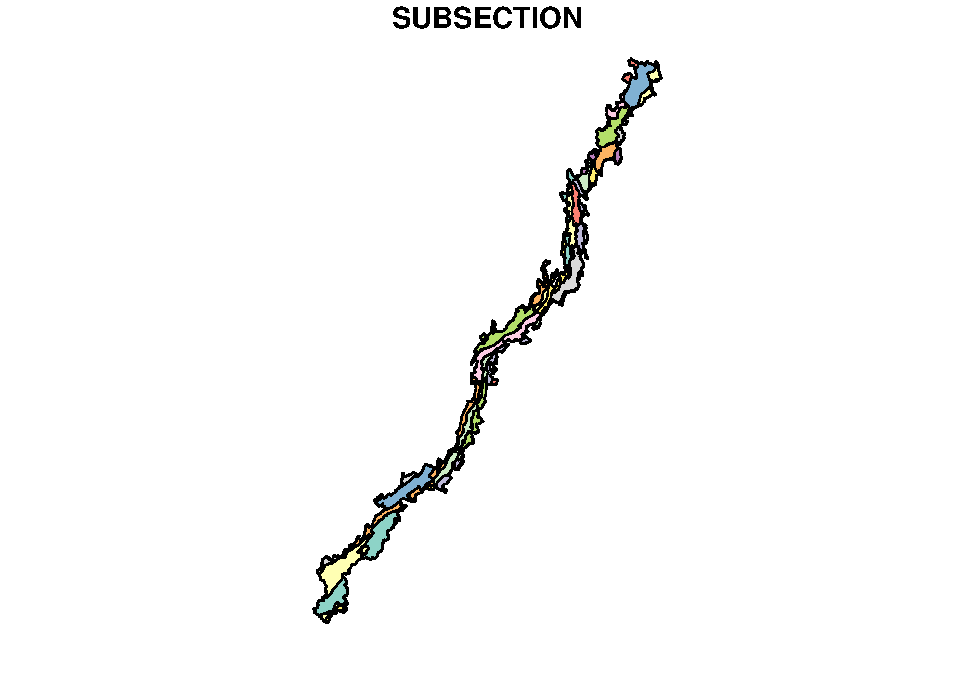
\includegraphics{_main_files/figure-latex/eco-subsections-1.pdf}

\begin{Shaded}
\begin{Highlighting}[]
\FunctionTok{plot}\NormalTok{(eco\_shapefile[}\StringTok{"SECTION\_NA"}\NormalTok{])}
\end{Highlighting}
\end{Shaded}

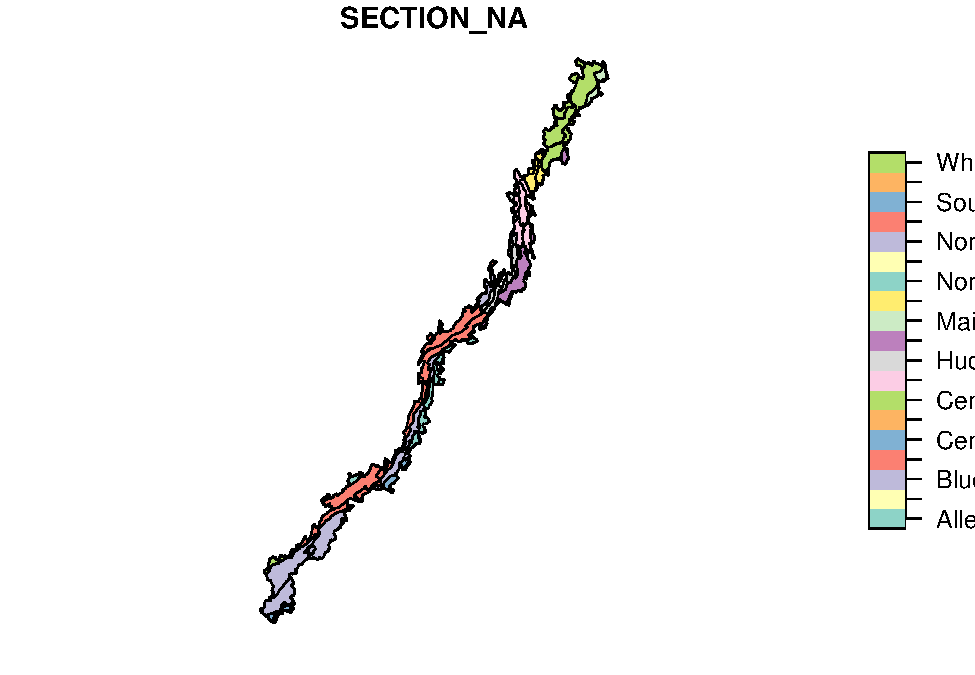
\includegraphics{_main_files/figure-latex/eco-subsections-2.pdf}

\begin{Shaded}
\begin{Highlighting}[]
\DocumentationTok{\#\# SUBSECTIONS:}
\FunctionTok{n\_distinct}\NormalTok{(eco\_shapefile}\SpecialCharTok{$}\NormalTok{SUBSECTION)}
\end{Highlighting}
\end{Shaded}

\begin{verbatim}
## [1] 50
\end{verbatim}

\begin{Shaded}
\begin{Highlighting}[]
\FunctionTok{levels}\NormalTok{(}\FunctionTok{as.factor}\NormalTok{(eco\_shapefile}\SpecialCharTok{$}\NormalTok{SUBSECTION))}
\end{Highlighting}
\end{Shaded}

\begin{verbatim}
##  [1] "211Aa"  "211Ba"  "211Bb"  "211Da"  "211Ec"  "211Fc"  "211Fd"  "211Ia" 
##  [9] "221Ae"  "221Al"  "221Am"  "221Ba"  "221Bb"  "221Bd"  "221Da"  "221Db" 
## [17] "221Dc"  "221Dd"  "221De"  "221Ja"  "221Jb"  "221Jc"  "231Ab"  "231Ac" 
## [25] "231Ad"  "231Ag"  "231Ib"  "M211Ab" "M211Ac" "M211Ad" "M211Ae" "M211Af"
## [33] "M211Ag" "M211Ba" "M211Bb" "M211Bc" "M211Ca" "M211Cb" "M211Cc" "M211Cd"
## [41] "M221Aa" "M221Ab" "M221Ac" "M221Ad" "M221Be" "M221Cb" "M221Da" "M221Db"
## [49] "M221Dc" "M221Dd"
\end{verbatim}

\begin{Shaded}
\begin{Highlighting}[]
\DocumentationTok{\#\# SUBSECTI\_1:}
\FunctionTok{levels}\NormalTok{(}\FunctionTok{as.factor}\NormalTok{(eco\_shapefile}\SpecialCharTok{$}\NormalTok{SUBSECTI\_1)) }
\end{Highlighting}
\end{Shaded}

\begin{verbatim}
##  [1] "Aroostook Hills"                         
##  [2] "Berkshire-Vermont Upland"                
##  [3] "Catskill Mountains"                      
##  [4] "Central Blue Ridge Mountains"            
##  [5] "Central Maine Embayment"                 
##  [6] "Central Maine Foothills"                 
##  [7] "Champlain Glacial Lake and Marine Plains"
##  [8] "Connecticut Lakes"                       
##  [9] "Eastern Allegheny Plateau"               
## [10] "Eastern Coal Fields"                     
## [11] "Gettysburg Piedmont Lowland"             
## [12] "Great Valley of Virginia"                
## [13] "Holston Valley"                          
## [14] "Hudson Highlands"                        
## [15] "Hudson Limestone Valley"                 
## [16] "Kittatinny-Shawangunk Ridges"            
## [17] "Lower Foot Hills"                        
## [18] "Lynchburg Belt"                          
## [19] "Mahoosic Rangely Lakes"                  
## [20] "Maine-New Brunswick Lowlands"            
## [21] "Maine Central Mountains"                 
## [22] "Metasedimentary Mountains"               
## [23] "Newark"                                  
## [24] "Northern Blue Ridge Mountains"           
## [25] "Northern Great Valley"                   
## [26] "Northern Green Mountain"                 
## [27] "Northern Piedmont"                       
## [28] "Northern Ridge and Valley"               
## [29] "Piedmont Ridge"                          
## [30] "Piedmont Upland"                         
## [31] "Pocono Plateau"                          
## [32] "Reading Prong"                           
## [33] "Ridge and Valley"                        
## [34] "Rolling Limestone Hills"                 
## [35] "Sandstone Hills"                         
## [36] "Schist Hills"                            
## [37] "Schist Plains"                           
## [38] "Sebago-Ossipee Hills and Plains"         
## [39] "Southern Blue Ridge Mountains"           
## [40] "Southern Green Mountain"                 
## [41] "Southern Piedmont"                       
## [42] "St. John Upland"                         
## [43] "Sunapee Uplands"                         
## [44] "Taconic Foothills"                       
## [45] "Taconic Mountains"                       
## [46] "Triassic Basins"                         
## [47] "Western Allegheny Mountain and Valley"   
## [48] "Western Maine Foothills"                 
## [49] "White Mountains"
\end{verbatim}

\begin{Shaded}
\begin{Highlighting}[]
\FunctionTok{n\_distinct}\NormalTok{(eco\_shapefile}\SpecialCharTok{$}\NormalTok{SUBSECTI\_1)}
\end{Highlighting}
\end{Shaded}

\begin{verbatim}
## [1] 49
\end{verbatim}

\begin{Shaded}
\begin{Highlighting}[]
\DocumentationTok{\#\# Note that \textquotesingle{}SUBSECTI\_1\textquotesingle{} names are not unique {-} there are two different "Northern Piedmont"}
\NormalTok{eco\_shapefile }\SpecialCharTok{\%\textgreater{}\%}
  \FunctionTok{filter}\NormalTok{(SUBSECTI\_1 }\SpecialCharTok{==} \StringTok{"Northern Piedmont"}\NormalTok{) }\SpecialCharTok{\%\textgreater{}\%}
  \FunctionTok{select}\NormalTok{(SUBSECTI\_1, SUBSECTION, SECTION\_NA, PROVINCE\_N) }\SpecialCharTok{\%\textgreater{}\%}
\NormalTok{  sf}\SpecialCharTok{::}\FunctionTok{st\_drop\_geometry}\NormalTok{() }
\end{Highlighting}
\end{Shaded}

\begin{verbatim}
## # A tibble: 2 x 4
##   SUBSECTI_1        SUBSECTION SECTION_NA                    PROVINCE_N         
## * <chr>             <chr>      <chr>                         <chr>              
## 1 Northern Piedmont M211Ba     New England Piedmont          Adirondack-New Eng~
## 2 Northern Piedmont 221De      Northern Appalachian Piedmont Eastern Broadleaf ~
\end{verbatim}

\begin{Shaded}
\begin{Highlighting}[]
\NormalTok{eco\_shapefile }\OtherTok{\textless{}{-}}\NormalTok{ eco\_shapefile }\SpecialCharTok{\%\textgreater{}\%}
  \FunctionTok{mutate}\NormalTok{(}\AttributeTok{SUBSECTI\_1 =} \FunctionTok{case\_when}\NormalTok{(}
\NormalTok{    SUBSECTI\_1 }\SpecialCharTok{==} \StringTok{"Northern Piedmont"} \SpecialCharTok{\&}\NormalTok{ SUBSECTION }\SpecialCharTok{==} \StringTok{"M211Ba"} \SpecialCharTok{\textasciitilde{}} \StringTok{"New Engl. Northern Piedmont"}\NormalTok{,}
\NormalTok{    SUBSECTI\_1 }\SpecialCharTok{==} \StringTok{"Northern Piedmont"} \SpecialCharTok{\&}\NormalTok{ SUBSECTION }\SpecialCharTok{==} \StringTok{"221De"} \SpecialCharTok{\textasciitilde{}} \StringTok{"Appal. Northern Piedmont"}\NormalTok{,}
    \AttributeTok{.default =} \FunctionTok{as.character}\NormalTok{(SUBSECTI\_1)))}
\end{Highlighting}
\end{Shaded}

Note that \texttt{SUBSECTI\_1} names are not unique. There are two different subsections both named ``Northern Piedmont''. See current re-name solution above.

\begin{Shaded}
\begin{Highlighting}[]
\DocumentationTok{\#\# Distinct SECTION\_NA:}
\FunctionTok{n\_distinct}\NormalTok{(eco\_shapefile}\SpecialCharTok{$}\NormalTok{SECTION\_NA)}
\end{Highlighting}
\end{Shaded}

\begin{verbatim}
## [1] 19
\end{verbatim}

\begin{Shaded}
\begin{Highlighting}[]
\FunctionTok{levels}\NormalTok{(}\FunctionTok{as.factor}\NormalTok{(eco\_shapefile}\SpecialCharTok{$}\NormalTok{SECTION\_NA))}
\end{Highlighting}
\end{Shaded}

\begin{verbatim}
##  [1] "Allegheny Mountains"                         
##  [2] "Aroostook Hills and Lowlands"                
##  [3] "Blue Ridge Mountains"                        
##  [4] "Catskill Mountains"                          
##  [5] "Central Appalachian Piedmont"                
##  [6] "Central Maine Coastal and Embayment"         
##  [7] "Central Ridge and Valley"                    
##  [8] "Green-Taconic-Berkshire Mountains"           
##  [9] "Hudson Valley"                               
## [10] "Lower New England"                           
## [11] "Maine - New Brunswick Foothills and Lowlands"
## [12] "New England Piedmont"                        
## [13] "Northern Appalachian Piedmont"               
## [14] "Northern Cumberland Mountains"               
## [15] "Northern Glaciated Allegheny Plateau"        
## [16] "Northern Ridge and Valley"                   
## [17] "Southern Appalachian Piedmont"               
## [18] "St. Lawrence and Champlain Valley"           
## [19] "White Mountains"
\end{verbatim}

\begin{Shaded}
\begin{Highlighting}[]
\DocumentationTok{\#\# Distinct PROVINCE\_N:}
\FunctionTok{n\_distinct}\NormalTok{(eco\_shapefile}\SpecialCharTok{$}\NormalTok{PROVINCE\_N)}
\end{Highlighting}
\end{Shaded}

\begin{verbatim}
## [1] 5
\end{verbatim}

\begin{Shaded}
\begin{Highlighting}[]
\FunctionTok{levels}\NormalTok{(}\FunctionTok{as.factor}\NormalTok{(eco\_shapefile}\SpecialCharTok{$}\NormalTok{PROVINCE\_N))}
\end{Highlighting}
\end{Shaded}

\begin{verbatim}
## [1] "Adirondack-New England Mixed Forest--Coniferous Forest--Alpine Meadow"
## [2] "Central Appalachian Broadleaf Forest-Coniferous Forest-Meadow"        
## [3] "Eastern Broadleaf Forest"                                             
## [4] "Northeastern Mixed Forest"                                            
## [5] "Southeastern Mixed Forest"
\end{verbatim}

\hypertarget{read-fia-data-into-r}{%
\section{Read FIA data into R}\label{read-fia-data-into-r}}

Load the FIA data stored locally (From ``\protect\hyperlink{download}{Download} Chapter) into R session.

\begin{Shaded}
\begin{Highlighting}[]
\DocumentationTok{\#\# load from default location (specified in 01{-}Download.Rmd chapter):}
\NormalTok{load\_default }\OtherTok{\textless{}{-}} \StringTok{\textquotesingle{}./download\_FIA/\textquotesingle{}} 
\DocumentationTok{\#\# Alternatively, enter specific custom location:}
\NormalTok{load\_custom }\OtherTok{\textless{}{-}} \StringTok{\textquotesingle{}C:/Users/JJGross/Documents/R\_projects/FIA\_data/allStates\textquotesingle{}}

\NormalTok{load\_location }\OtherTok{\textless{}{-}}\NormalTok{ load\_custom}
\CommentTok{\#load\_location \textless{}{-} load\_default}

\DocumentationTok{\#\# Change number of processing cores used, if desired}
\NormalTok{cores }\OtherTok{\textless{}{-}}\NormalTok{ parallel}\SpecialCharTok{::}\FunctionTok{detectCores}\NormalTok{(}\AttributeTok{logical =} \ConstantTok{FALSE}\NormalTok{)}\SpecialCharTok{{-}}\DecValTok{2} 
\end{Highlighting}
\end{Shaded}

Read the FIA data stored locally (From ``\protect\hyperlink{download}{Download} Chapter) using the \href{https://rdrr.io/cran/rFIA/man/readFIA.html}{ReadFIA()} function.

\begin{Shaded}
\begin{Highlighting}[]
\DocumentationTok{\#\# Specify the 13 APPA states by state code (this is extra insurance that the wrong states are not loaded, if other states have been downloaded to same directory)}
\NormalTok{at\_states }\OtherTok{\textless{}{-}} \FunctionTok{c}\NormalTok{(}\StringTok{\textquotesingle{}CT\textquotesingle{}}\NormalTok{, }\StringTok{\textquotesingle{}GA\textquotesingle{}}\NormalTok{, }\StringTok{\textquotesingle{}ME\textquotesingle{}}\NormalTok{, }\StringTok{\textquotesingle{}MD\textquotesingle{}}\NormalTok{, }\StringTok{\textquotesingle{}MA\textquotesingle{}}\NormalTok{, }
               \StringTok{\textquotesingle{}NH\textquotesingle{}}\NormalTok{, }\StringTok{\textquotesingle{}NJ\textquotesingle{}}\NormalTok{, }\StringTok{\textquotesingle{}NY\textquotesingle{}}\NormalTok{, }\StringTok{\textquotesingle{}NC\textquotesingle{}}\NormalTok{, }\StringTok{\textquotesingle{}PA\textquotesingle{}}\NormalTok{, }
               \StringTok{\textquotesingle{}TN\textquotesingle{}}\NormalTok{, }\StringTok{\textquotesingle{}VT\textquotesingle{}}\NormalTok{, }\StringTok{\textquotesingle{}VA\textquotesingle{}}\NormalTok{)}

\DocumentationTok{\#\# Read FIA data }
\NormalTok{at\_states\_FIA }\OtherTok{\textless{}{-}} \FunctionTok{readFIA}\NormalTok{(}\AttributeTok{dir =}\NormalTok{ load\_location, }\AttributeTok{states =}\NormalTok{ at\_states, }\AttributeTok{nCores =}\NormalTok{ cores)}
\end{Highlighting}
\end{Shaded}

\hypertarget{clip-fia-plots-by-ecoregion}{%
\section{Clip FIA plots by Ecoregion}\label{clip-fia-plots-by-ecoregion}}

\href{https://rdrr.io/cran/rFIA/man/clipFIA.html}{clipFIA()} performs space-time queries on Forest Inventory and Analysis Database (FIADB). \texttt{clipFIA} subsets the dataset to include only data associated with particular inventory years (i.e., most recent), and/or only data within a user-defined region.

Spatially, the \texttt{mask\ =\ eco} argument below selects only the \texttt{at\_states\_FIA} FIA plots which fall within the perimeter of the \texttt{eco} spatial extent (i.e.~the outer boundary of the ecoregion polygons).

Temporally, the \texttt{mostRecent} argument returns only data for most recent inventory if set to \texttt{TRUE}

\begin{Shaded}
\begin{Highlighting}[]
\DocumentationTok{\#\# Restrict to most recent inventory}
\NormalTok{at\_FIA\_MR }\OtherTok{\textless{}{-}} \FunctionTok{clipFIA}\NormalTok{(at\_states\_FIA, }\AttributeTok{matchEval =} \ConstantTok{TRUE}\NormalTok{, }\AttributeTok{mostRecent =} \ConstantTok{TRUE}\NormalTok{, }\AttributeTok{mask =}\NormalTok{ eco\_shapefile)}
\FunctionTok{saveRDS}\NormalTok{(at\_FIA\_MR, }\AttributeTok{file =} \FunctionTok{paste0}\NormalTok{(save\_location, }\StringTok{"at\_FIA\_MR.rds"}\NormalTok{))}

\DocumentationTok{\#\# Access all inventories}
\NormalTok{at\_FIA }\OtherTok{\textless{}{-}} \FunctionTok{clipFIA}\NormalTok{(at\_states\_FIA, }\AttributeTok{matchEval =} \ConstantTok{TRUE}\NormalTok{, }\AttributeTok{mostRecent =} \ConstantTok{FALSE}\NormalTok{, }\AttributeTok{mask =}\NormalTok{ eco\_shapefile)}
\FunctionTok{saveRDS}\NormalTok{(at\_FIA, }\AttributeTok{file =} \FunctionTok{paste0}\NormalTok{(save\_location, }\StringTok{"at\_FIA.rds"}\NormalTok{))}
\end{Highlighting}
\end{Shaded}

Note the argument \texttt{matchEval\ =\ TRUE} in the above function. The \href{https://rdrr.io/cran/rFIA/man/clipFIA.html}{clipFIA()} documentation states that:

\begin{quote}
``if \texttt{matchEval\ =\ TRUE}, \texttt{clipFIA()} returns a subset of data for which there are matching reporting years across
states. Only useful if db contains multiple state subsets of the FIA database.''
\end{quote}

This seems appropriate for the Appalachian Trail dataset, but when compared (12 March 2024), both \texttt{matchEval\ =\ TRUE} and \texttt{matchEval\ =\ FALSE} appeared to result in the same output. This may have something to do with the method that is used (e.g.~`Annual'``\,' vs `TI'). Further evaluation is needed.

Note that currently matchEval argument is set to \texttt{matchEval\ =\ TRUE} for both \texttt{at\_FIA} and \texttt{at\_FIA\_MR}. Confirm this is appropriate.

\hypertarget{ecosubsections}{%
\subsection{Ecosubsections}\label{ecosubsections}}

It is important to note the column \texttt{ECOSUBCD} which is part of the native FIA database and referenced in the \href{https://www.fs.usda.gov/research/understory/forest-inventory-and-analysis-database-user-guide-phase-2}{FIA Database User Guide}. The \texttt{ECOSUBCD} column can be included in the output of most \texttt{rFIA} functions with the argument \texttt{grpBy\ =\ c(ECOSUBCD)}. The FIA database guide states that subsection codes for the conterminous United States were developed as part of the ``Ecological Subregions: Sections and Subsections for the Conterminous United States'' publication (Cleland et al.~2007).

Conversely, the same ecoregional subsection code can be found within the \texttt{APPA\_Ecoregions\_USFS\_HUC10\_Shell\_AEA} shapefile column \texttt{eco\$SUBSECTION} along with additional related columns - for example, the full subsection name in the \texttt{SUBSECTI\_1} column. These columns (and others added below) are appended to the FIA dataset during most rFIA functions by way of the \texttt{polys\ =\ eco}. For this reason the \texttt{polys\ =\ eco}argument is often more advantageous than the \texttt{grpBy\ =\ c(ECOSUBCD)} and the \texttt{polys\ =\ eco}argument is utilized throughout the make.Rmd chapter.

Note that this \texttt{polys\ =\ eco} argument is different than the \texttt{rFIA::clipFIA(mask\ =\ eco)} function/argument which only clips the plot data by the eco mask (outer spatial boundary) and does not append any data.

\hypertarget{supporting-tables}{%
\section{Supporting tables}\label{supporting-tables}}

\hypertarget{appalachian-trail-spatial-centerline-data}{%
\subsection{Appalachian trail spatial centerline data}\label{appalachian-trail-spatial-centerline-data}}

\begin{Shaded}
\begin{Highlighting}[]
\DocumentationTok{\#\# Manually downloaded \textasciigrave{}Appalachian\_National\_Scenic\_Trail.shp\textasciigrave{} from \textasciigrave{}APPAForesthealthReport\textasciigrave{} repo. }
\NormalTok{centerline\_shapefile\_location }\OtherTok{\textless{}{-}} \StringTok{"move\_to\_server/at\_centerline/"} 

\DocumentationTok{\#\# read in shapefile of Appalachian trail center{-}line}
\NormalTok{ at\_centerline }\OtherTok{\textless{}{-}}\NormalTok{ sf}\SpecialCharTok{::}\FunctionTok{st\_read}\NormalTok{(}\FunctionTok{paste0}\NormalTok{(centerline\_shapefile\_location, }\StringTok{"Appalachian\_National\_Scenic\_Trail.shp"}\NormalTok{)) }\SpecialCharTok{\%\textgreater{}\%}
   \FunctionTok{mutate}\NormalTok{(}\AttributeTok{region\_3cl =} \FunctionTok{case\_when}\NormalTok{(}
\NormalTok{     Region }\SpecialCharTok{==} \StringTok{"New England"} \SpecialCharTok{\textasciitilde{}} \StringTok{"Northeast"}\NormalTok{,}
\NormalTok{     Region }\SpecialCharTok{==} \StringTok{"Mid{-}Atlantic"} \SpecialCharTok{\textasciitilde{}} \StringTok{"Mid{-}Atlantic"}\NormalTok{,}
\NormalTok{     Region }\SpecialCharTok{\%in\%} \FunctionTok{c}\NormalTok{(}\StringTok{"Southern"}\NormalTok{, }\StringTok{"Virginia"}\NormalTok{) }\SpecialCharTok{\textasciitilde{}} \StringTok{"Southeast"}
\NormalTok{   ))}

\FunctionTok{saveRDS}\NormalTok{(at\_centerline, }\FunctionTok{paste0}\NormalTok{(save\_location, }\StringTok{"at\_centerline.rds"}\NormalTok{))}
\end{Highlighting}
\end{Shaded}

\texttt{Appalachian\_National\_Scenic\_Trail.shp} currently saved within \texttt{APPAForesthealthReport} repo. In future move this to appropriate location (e.g.~IRMA).

\hypertarget{appa-fia-plots}{%
\subsection{APPA FIA plots}\label{appa-fia-plots}}

Note that the \texttt{rFIA::tpa()} function was used below to calculate and construct tables for APPA FIA plot-level attributes (e.g.~elevation, etc.). TPA was selected because it is a core metric of FIA methods and should be present in all field visited plots.

\begin{Shaded}
\begin{Highlighting}[]
\DocumentationTok{\#\# Get plot{-}level data for the most recent tpa dataset}
\NormalTok{tpa\_plots\_MR }\OtherTok{\textless{}{-}}\NormalTok{ rFIA}\SpecialCharTok{::}\FunctionTok{tpa}\NormalTok{(at\_FIA\_MR, }
                          \AttributeTok{byPlot =} \ConstantTok{TRUE}\NormalTok{, }
                          \AttributeTok{grpBy =} \FunctionTok{c}\NormalTok{(STATECD, ECOSUBCD, ELEV),}
                          \AttributeTok{returnSpatial =} \ConstantTok{TRUE}\NormalTok{) }

\DocumentationTok{\#\# Get plot{-}level data for full tpa dataset  }
\NormalTok{tpa\_plots }\OtherTok{\textless{}{-}}\NormalTok{ rFIA}\SpecialCharTok{::}\FunctionTok{tpa}\NormalTok{(at\_FIA, }
                       \AttributeTok{byPlot =} \ConstantTok{TRUE}\NormalTok{, }
                       \AttributeTok{grpBy =} \FunctionTok{c}\NormalTok{(STATECD, ECOSUBCD, ELEV),}
                       \AttributeTok{returnSpatial =} \ConstantTok{TRUE}\NormalTok{) }

\DocumentationTok{\#\# Get only the unique plot locations (pltID)}
\DocumentationTok{\#\# i.e. exclude the revisits }
\NormalTok{tpa\_plots\_by\_year }\OtherTok{\textless{}{-}}\NormalTok{ tpa\_plots }\SpecialCharTok{|\textgreater{}}
  \CommentTok{\# HAVE TO DO BIND ROWS HERE BECAUSE \textasciigrave{}tpa\_plots\textquotesingle{} SUPRISINGLY DOES NOT }
  \CommentTok{\# CONTAIN ALL PLOTS FOUND IN \textasciigrave{}tpa\_plots\_MR\textquotesingle{}.}
  \CommentTok{\# Error with rFIA discussed below}
\NormalTok{  dplyr}\SpecialCharTok{::}\FunctionTok{bind\_rows}\NormalTok{(tpa\_plots\_MR) }\SpecialCharTok{|\textgreater{}}
\NormalTok{  dplyr}\SpecialCharTok{::}\FunctionTok{group\_by}\NormalTok{(PLT\_CN) }\SpecialCharTok{|\textgreater{}} \CommentTok{\#PLT\_CN is each unique event, while pltID is each unique plot location}
  \FunctionTok{distinct}\NormalTok{()}

\DocumentationTok{\#\# Get only the unique plot locations (pltID)}
\DocumentationTok{\#\# i.e. exclude the revisits }
\NormalTok{tpa\_plots\_distinct }\OtherTok{\textless{}{-}}\NormalTok{ tpa\_plots\_by\_year }\SpecialCharTok{|\textgreater{}}
  \FunctionTok{select}\NormalTok{(pltID, STATECD, ECOSUBCD, ELEV, geometry) }\SpecialCharTok{\%\textgreater{}\%}
  \FunctionTok{distinct}\NormalTok{()}
\end{Highlighting}
\end{Shaded}

Display APPA FIA plots by eco-subsection and southern most plot used to calculated distance.

\begin{Shaded}
\begin{Highlighting}[]
\DocumentationTok{\#\# Select Southern{-}most plot}
\NormalTok{most\_S\_plot }\OtherTok{\textless{}{-}}\NormalTok{ tpa\_plots\_distinct }\SpecialCharTok{\%\textgreater{}\%}
  \FunctionTok{filter}\NormalTok{(pltID }\SpecialCharTok{==} \StringTok{"5\_13\_85\_5"}\NormalTok{)}

\DocumentationTok{\#\# ecosubsection colors}
\NormalTok{ecosubCol }\OtherTok{\textless{}{-}} \FunctionTok{colorFactor}\NormalTok{(}\FunctionTok{rainbow}\NormalTok{(}\DecValTok{51}\NormalTok{), tpa\_plots\_distinct}\SpecialCharTok{$}\NormalTok{ECOSUBCD)}
\DocumentationTok{\#\# leaflet map}
\NormalTok{tpa\_plots\_distinct }\SpecialCharTok{\%\textgreater{}\%}  
  \FunctionTok{leaflet}\NormalTok{() }\SpecialCharTok{\%\textgreater{}\%}
  \FunctionTok{addTiles}\NormalTok{() }\SpecialCharTok{\%\textgreater{}\%}
  \FunctionTok{addCircleMarkers}\NormalTok{(}
    \AttributeTok{color =} \SpecialCharTok{\textasciitilde{}}\FunctionTok{ecosubCol}\NormalTok{(ECOSUBCD),}
    \AttributeTok{stroke =} \ConstantTok{FALSE}\NormalTok{, }\AttributeTok{fillOpacity =} \DecValTok{1}\NormalTok{,}
    \AttributeTok{radius =} \DecValTok{4}\NormalTok{) }\SpecialCharTok{\%\textgreater{}\%}
  \FunctionTok{addMarkers}\NormalTok{(}\AttributeTok{data =}\NormalTok{ most\_S\_plot)}
\end{Highlighting}
\end{Shaded}

\begin{verbatim}
## Google Chrome was not found. Try setting the `CHROMOTE_CHROME` environment variable to the executable of a Chromium-based browser, such as Google Chrome, Chromium or Brave.
\end{verbatim}

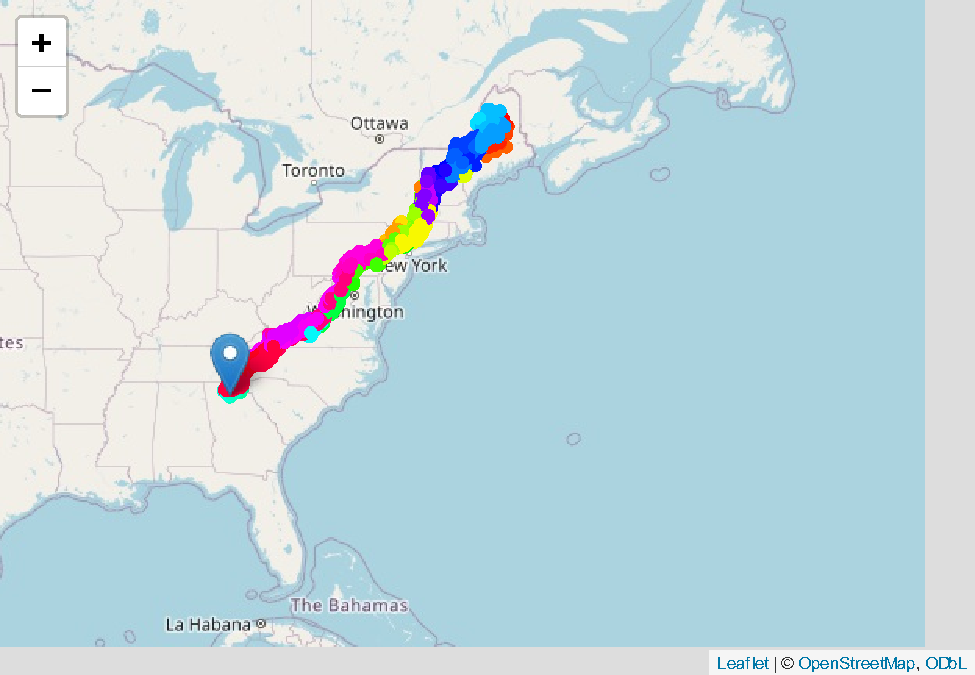
\includegraphics{_main_files/figure-latex/plot-map-southpoint-1.pdf}
Calculate each plot's distance from southern point for use in displaying data as transect along axis.

\begin{Shaded}
\begin{Highlighting}[]
\NormalTok{tpa\_plots\_distance }\OtherTok{\textless{}{-}}\NormalTok{ tpa\_plots\_distinct }\SpecialCharTok{|\textgreater{}}
  \FunctionTok{mutate}\NormalTok{(}\AttributeTok{S\_plot =}\NormalTok{ most\_S\_plot}\SpecialCharTok{$}\NormalTok{geometry) }\SpecialCharTok{|\textgreater{}} \CommentTok{\# add south point}
  \FunctionTok{mutate}\NormalTok{(}\AttributeTok{dist\_unit =}\NormalTok{ sf}\SpecialCharTok{::}\FunctionTok{st\_distance}\NormalTok{(}
\NormalTok{    S\_plot, geometry, }\AttributeTok{by\_element =} \ConstantTok{TRUE}\NormalTok{)) }\SpecialCharTok{|\textgreater{}} \CommentTok{\# calculate distance}
  \FunctionTok{mutate}\NormalTok{(}\AttributeTok{distance\_m =} \FunctionTok{round}\NormalTok{(}\FunctionTok{as.numeric}\NormalTok{(dist\_unit))) }\SpecialCharTok{|\textgreater{}}
  \FunctionTok{select}\NormalTok{(}\SpecialCharTok{{-}}\NormalTok{S\_plot, }\SpecialCharTok{{-}}\NormalTok{dist\_unit)}

\DocumentationTok{\#\# Create a continuous palette function}
\NormalTok{dist\_pal }\OtherTok{\textless{}{-}} \FunctionTok{colorNumeric}\NormalTok{(}\AttributeTok{palette =} \StringTok{"Blues"}\NormalTok{, }\AttributeTok{domain =}\NormalTok{ tpa\_plots\_distance}\SpecialCharTok{$}\NormalTok{distance\_m)}
\DocumentationTok{\#\# leaflet map}
\NormalTok{tpa\_plots\_distance }\SpecialCharTok{\%\textgreater{}\%}  
  \FunctionTok{leaflet}\NormalTok{() }\SpecialCharTok{\%\textgreater{}\%}
  \FunctionTok{addTiles}\NormalTok{() }\SpecialCharTok{\%\textgreater{}\%}
  \FunctionTok{addCircleMarkers}\NormalTok{(}
    \AttributeTok{color =} \SpecialCharTok{\textasciitilde{}}\FunctionTok{dist\_pal}\NormalTok{(distance\_m),}
    \AttributeTok{stroke =} \ConstantTok{FALSE}\NormalTok{, }\AttributeTok{fillOpacity =} \DecValTok{1}\NormalTok{,}
    \AttributeTok{radius =} \DecValTok{4}\NormalTok{) }\SpecialCharTok{\%\textgreater{}\%}
  \FunctionTok{addMarkers}\NormalTok{(}\AttributeTok{data =}\NormalTok{ most\_S\_plot)}
\end{Highlighting}
\end{Shaded}

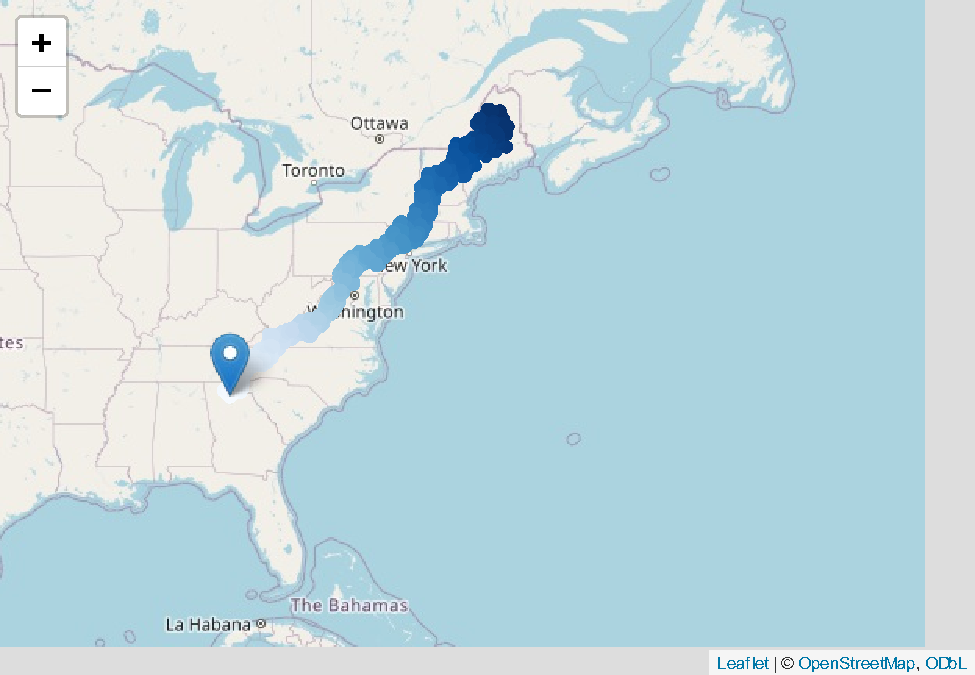
\includegraphics{_main_files/figure-latex/calc-plot-dist-1.pdf}

Demo usage of plot attributes

\begin{Shaded}
\begin{Highlighting}[]
\NormalTok{plot\_attributes }\OtherTok{\textless{}{-}}\NormalTok{ tpa\_plots\_distance}

\CommentTok{\# Demo plot distance x elevation}
\NormalTok{plot\_attributes }\SpecialCharTok{|\textgreater{}}
  \FunctionTok{group\_by}\NormalTok{(ECOSUBCD)}\SpecialCharTok{|\textgreater{}}
  \FunctionTok{mutate}\NormalTok{(}\AttributeTok{median\_dist =} \FunctionTok{median}\NormalTok{(distance\_m)) }\SpecialCharTok{|\textgreater{}}
  \FunctionTok{mutate}\NormalTok{(}\AttributeTok{median\_elev =} \FunctionTok{median}\NormalTok{(ELEV)) }\SpecialCharTok{|\textgreater{}}
  \FunctionTok{ggplot}\NormalTok{(}\FunctionTok{aes}\NormalTok{(}\AttributeTok{x=} \FunctionTok{fct\_reorder}\NormalTok{(ECOSUBCD, distance\_m), }
             \AttributeTok{y=}\NormalTok{ELEV, }
             \AttributeTok{fill =} \FunctionTok{as.factor}\NormalTok{(median\_elev))) }\SpecialCharTok{+}
  \FunctionTok{geom\_boxplot}\NormalTok{() }\SpecialCharTok{+}
  \FunctionTok{theme}\NormalTok{(}\AttributeTok{axis.text.x =} \FunctionTok{element\_text}\NormalTok{(}\AttributeTok{angle =} \DecValTok{90}\NormalTok{, }\AttributeTok{vjust =} \FloatTok{0.5}\NormalTok{, }\AttributeTok{hjust=}\DecValTok{1}\NormalTok{),}
        \AttributeTok{legend.position =} \StringTok{\textquotesingle{}none\textquotesingle{}}\NormalTok{) }\SpecialCharTok{+}
  \FunctionTok{xlab}\NormalTok{(}\StringTok{"Ecosubsection (from SW to NE)"}\NormalTok{) }\SpecialCharTok{+} \FunctionTok{ylab}\NormalTok{(}\StringTok{"Plot Elevation"}\NormalTok{) }
\end{Highlighting}
\end{Shaded}

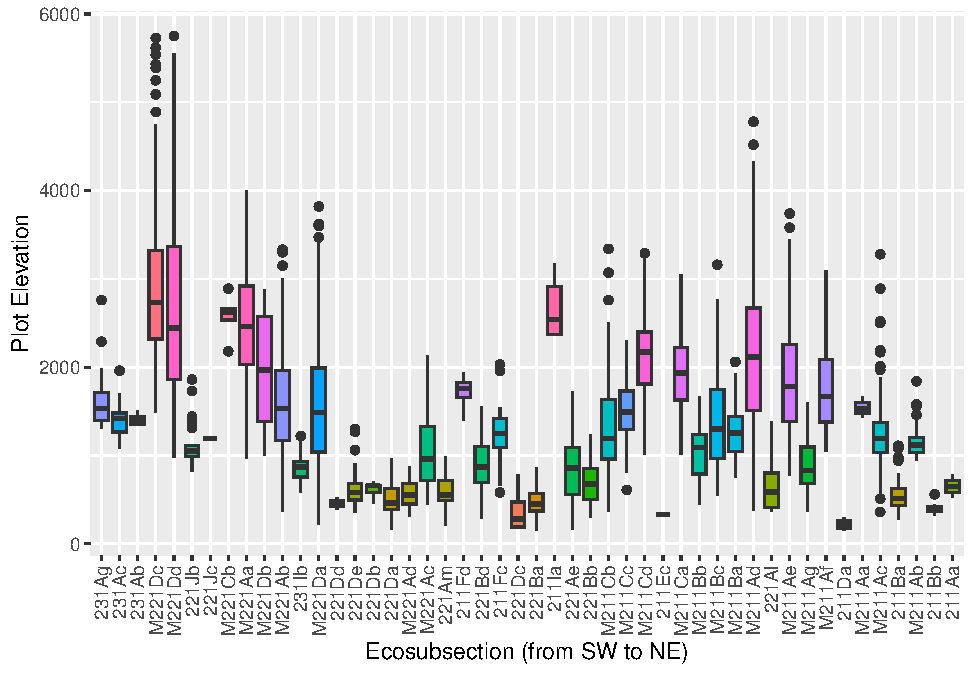
\includegraphics{_main_files/figure-latex/plot-attributes-1.pdf}

\hypertarget{check-plot-counts}{%
\subsubsection{Check Plot Counts}\label{check-plot-counts}}

Perform some checks on records within tpa dataset - helps gauge dataset changes. Can also add quality assurance checks here:

\begin{Shaded}
\begin{Highlighting}[]
\DocumentationTok{\#\# Check that entire dataset (at\_plots) contains most recent dataset (at\_plots\_MR) }
\NormalTok{tpa\_chk }\OtherTok{\textless{}{-}}\NormalTok{ sf}\SpecialCharTok{::}\FunctionTok{st\_drop\_geometry}\NormalTok{(tpa\_plots)}
\NormalTok{tpa\_chk\_MR }\OtherTok{\textless{}{-}}\NormalTok{ sf}\SpecialCharTok{::}\FunctionTok{st\_drop\_geometry}\NormalTok{(tpa\_plots\_MR)}

\NormalTok{MRplots\_not\_in\_full\_tpa\_dataset }\OtherTok{\textless{}{-}} \FunctionTok{anti\_join}\NormalTok{(tpa\_chk\_MR, tpa\_chk, }\AttributeTok{by =} \FunctionTok{join\_by}\NormalTok{(pltID))}
\ControlFlowTok{if}\NormalTok{ (}\FunctionTok{nrow}\NormalTok{(MRplots\_not\_in\_full\_tpa\_dataset) }\SpecialCharTok{!=} \DecValTok{0}\NormalTok{) \{}
  \FunctionTok{warning}\NormalTok{(}\StringTok{"tpa\_plots does not contain all plots found in tpa\_plots\_MR (most recent) dataset"}\NormalTok{)}
\NormalTok{\}}
\end{Highlighting}
\end{Shaded}

\begin{verbatim}
## Warning: tpa_plots does not contain all plots found in tpa_plots_MR (most
## recent) dataset
\end{verbatim}

\begin{Shaded}
\begin{Highlighting}[]
\DocumentationTok{\#\# total events/visits}
\NormalTok{tpa\_event\_count }\OtherTok{\textless{}{-}} \FunctionTok{nrow}\NormalTok{(tpa\_chk) }
\NormalTok{tpa\_event\_count }\CommentTok{\# 12,457}
\end{Highlighting}
\end{Shaded}

\begin{verbatim}
## [1] 12457
\end{verbatim}

\begin{Shaded}
\begin{Highlighting}[]
\DocumentationTok{\#\# total plot locations}
\NormalTok{tpa\_plot\_count }\OtherTok{\textless{}{-}} \FunctionTok{length}\NormalTok{(}\FunctionTok{unique}\NormalTok{(tpa\_chk}\SpecialCharTok{$}\NormalTok{pltID)) }
\NormalTok{tpa\_plot\_count }\CommentTok{\# 4,328}
\end{Highlighting}
\end{Shaded}

\begin{verbatim}
## [1] 4328
\end{verbatim}

\begin{Shaded}
\begin{Highlighting}[]
\NormalTok{tpa\_plots\_summary }\OtherTok{\textless{}{-}}\NormalTok{ tpa\_chk }\SpecialCharTok{|\textgreater{}}
  \FunctionTok{group\_by}\NormalTok{(pltID) }\SpecialCharTok{|\textgreater{}}
  \FunctionTok{summarise}\NormalTok{(}\AttributeTok{visits =} \FunctionTok{n}\NormalTok{()) }\SpecialCharTok{|\textgreater{}}
  \FunctionTok{group\_by}\NormalTok{(visits) }\SpecialCharTok{|\textgreater{}}
  \FunctionTok{summarize}\NormalTok{(}\AttributeTok{n\_plots =} \FunctionTok{n}\NormalTok{())}

\NormalTok{tpa\_plots\_summary}
\end{Highlighting}
\end{Shaded}

\begin{verbatim}
## # A tibble: 5 x 2
##   visits n_plots
##    <int>   <int>
## 1      1     571
## 2      2     781
## 3      3    1590
## 4      4    1376
## 5      5      10
\end{verbatim}

\begin{Shaded}
\begin{Highlighting}[]
\DocumentationTok{\#\# In 2022 }
\CommentTok{\#      1     571 (571 plots measured once)}
\CommentTok{\#      2     781 (781 plots measured twice)}
\CommentTok{\#      3    1590}
\CommentTok{\#      4    1376}
\CommentTok{\#      5      10}

\DocumentationTok{\#\# total events/visits}
\NormalTok{tpa\_event\_count\_MR }\OtherTok{\textless{}{-}} \FunctionTok{nrow}\NormalTok{(tpa\_chk\_MR) }
\NormalTok{tpa\_event\_count\_MR }\CommentTok{\# 3,980}
\end{Highlighting}
\end{Shaded}

\begin{verbatim}
## [1] 3980
\end{verbatim}

\begin{Shaded}
\begin{Highlighting}[]
\DocumentationTok{\#\# total plot locations}
\NormalTok{tpa\_plot\_count\_MR }\OtherTok{\textless{}{-}} \FunctionTok{length}\NormalTok{(}\FunctionTok{unique}\NormalTok{(tpa\_chk\_MR}\SpecialCharTok{$}\NormalTok{pltID)) }
\NormalTok{tpa\_plot\_count\_MR }\CommentTok{\# 3,980}
\end{Highlighting}
\end{Shaded}

\begin{verbatim}
## [1] 3980
\end{verbatim}

\begin{Shaded}
\begin{Highlighting}[]
\ControlFlowTok{if}\NormalTok{ (tpa\_event\_count\_MR }\SpecialCharTok{!=}\NormalTok{ tpa\_plot\_count\_MR) \{}
  \FunctionTok{warning}\NormalTok{(}\StringTok{"some plots not unique in most recent (MR) dataset"}\NormalTok{)}
\NormalTok{\}}
\end{Highlighting}
\end{Shaded}

Possible error with rFIA: tpa\_plots (full dataset) does not contain all plots found in tpa\_plots\_MR (most recent) dataset'' see \texttt{MRplots\_not\_in\_full\_tpa\_dataset} for table of missing plots.

\hypertarget{subsections}{%
\subsection{Subsections}\label{subsections}}

\hypertarget{check-subsections}{%
\subsubsection{Check subsections}\label{check-subsections}}

\begin{Shaded}
\begin{Highlighting}[]
\NormalTok{tpa\_ECOSUBCD\_distinct }\OtherTok{\textless{}{-}}\NormalTok{ tpa\_plots\_distinct }\SpecialCharTok{|\textgreater{}}
\NormalTok{  sf}\SpecialCharTok{::}\FunctionTok{st\_drop\_geometry}\NormalTok{() }\SpecialCharTok{|\textgreater{}}
  \FunctionTok{distinct}\NormalTok{(ECOSUBCD)}

\DocumentationTok{\#\# Eco shapefile:}
\NormalTok{eco }\OtherTok{\textless{}{-}}\NormalTok{ eco\_shapefile }\SpecialCharTok{\%\textgreater{}\%}
  \FunctionTok{full\_join}\NormalTok{(tpa\_ECOSUBCD\_distinct, }\AttributeTok{by =} \FunctionTok{c}\NormalTok{(}\StringTok{"SUBSECTION"} \OtherTok{=} \StringTok{"ECOSUBCD"}\NormalTok{)) }\SpecialCharTok{\%\textgreater{}\%}
\NormalTok{  sf}\SpecialCharTok{::}\FunctionTok{st\_transform}\NormalTok{(}\StringTok{\textquotesingle{}+proj=longlat +datum=WGS84\textquotesingle{}}\NormalTok{)}

\DocumentationTok{\#\# return all rows from eco\_shapefile without a match in FIA\_plots}
\DocumentationTok{\#\# These are subsections with no FIA plots:}
\NormalTok{dplyr}\SpecialCharTok{::}\FunctionTok{anti\_join}\NormalTok{(eco, tpa\_ECOSUBCD\_distinct, }\AttributeTok{by =} \FunctionTok{join\_by}\NormalTok{(SUBSECTION }\SpecialCharTok{==}\NormalTok{ ECOSUBCD))}
\end{Highlighting}
\end{Shaded}

\begin{verbatim}
## Simple feature collection with 3 features and 15 fields
## Geometry type: MULTIPOLYGON
## Dimension:     XY
## Bounding box:  xmin: -83.99575 ymin: 34.51386 xmax: -80.44353 ymax: 37.65403
## Geodetic CRS:  +proj=longlat +datum=WGS84
## # A tibble: 3 x 16
##      AREA PERIMETER ECOMAP_200 ECOMAP_201 PROVINCE SECTION SUBSECTION DOMAIN_NAM
##     <dbl>     <dbl>      <int>      <int> <chr>    <chr>   <chr>      <chr>     
## 1  7.42e8   436121.       1232       1381 M221     M221B   M221Be     Humid Tem~
## 2  3.99e4  1265905.       1480       1590 221      221J    221Ja      Humid Tem~
## 3  2.10e6   415055.       1688       1746 231      231A    231Ad      Humid Tem~
## # i 8 more variables: DIVISION_N <chr>, PROVINCE_N <chr>, SECTION_NA <chr>,
## #   SUBSECTI_1 <chr>, ATIntersec <int>, Acres <dbl>, Hectares <dbl>,
## #   geometry <MULTIPOLYGON [°]>
\end{verbatim}

\begin{Shaded}
\begin{Highlighting}[]
\DocumentationTok{\#\# return all rows from FIA\_plots without a match in eco\_shapefile}
\DocumentationTok{\#\# These rows are locations with FIA plots but no subsection included in shapefile:}
\NormalTok{eco }\SpecialCharTok{\%\textgreater{}\%} \FunctionTok{filter}\NormalTok{(}\FunctionTok{is.na}\NormalTok{(SECTION)) }
\end{Highlighting}
\end{Shaded}

\begin{verbatim}
## Simple feature collection with 1 feature and 15 fields (with 1 geometry empty)
## Geometry type: MULTIPOLYGON
## Dimension:     XY
## Bounding box:  xmin: NA ymin: NA xmax: NA ymax: NA
## Geodetic CRS:  +proj=longlat +datum=WGS84
## # A tibble: 1 x 16
##    AREA PERIMETER ECOMAP_200 ECOMAP_201 PROVINCE SECTION SUBSECTION DOMAIN_NAM
## * <dbl>     <dbl>      <int>      <int> <chr>    <chr>   <chr>      <chr>     
## 1    NA        NA         NA         NA <NA>     <NA>    M211Aa     <NA>      
## # i 8 more variables: DIVISION_N <chr>, PROVINCE_N <chr>, SECTION_NA <chr>,
## #   SUBSECTI_1 <chr>, ATIntersec <int>, Acres <dbl>, Hectares <dbl>,
## #   geometry <MULTIPOLYGON [°]>
\end{verbatim}

\hypertarget{missing-ecosubsection-info}{%
\subsubsection{Missing eco\$SUBSECTION info}\label{missing-ecosubsection-info}}

Note that \texttt{eco} shapefile is missing information for SUBSECTION \texttt{M211Aa\ -\ International\ Boundary\ Plateau}. This needs to be fixed in original shapefile.

Temporary fix here:

\begin{Shaded}
\begin{Highlighting}[]
\DocumentationTok{\#\# missing info found by google search of "M211Aa"}
\CommentTok{\# https://www.fs.usda.gov/research/publications/misc/73326{-}wo{-}gtr{-}76d{-}cleland2007.pdf}
\NormalTok{missing\_subsection }\OtherTok{\textless{}{-}} \FunctionTok{data.frame}\NormalTok{(}
  \AttributeTok{PROVINCE =} \StringTok{"M211"}\NormalTok{, }
  \AttributeTok{SECTION =} \StringTok{"M211A"}\NormalTok{, }
  \AttributeTok{SUBSECTION =} \StringTok{"M211Aa"}\NormalTok{, }
  \AttributeTok{SECTION\_NA =} \StringTok{"White Mountains"}\NormalTok{,}
  \AttributeTok{SUBSECTI\_1 =} \StringTok{"International Boundary Plateau"}\NormalTok{)}

\NormalTok{eco }\OtherTok{\textless{}{-}}\NormalTok{ eco }\SpecialCharTok{|\textgreater{}}
  \FunctionTok{filter}\NormalTok{(SUBSECTION }\SpecialCharTok{!=} \StringTok{"M211Aa"}\NormalTok{) }\SpecialCharTok{|\textgreater{}}
  \FunctionTok{bind\_rows}\NormalTok{(missing\_subsection)}
\end{Highlighting}
\end{Shaded}

\hypertarget{calculate-n-plots}{%
\subsubsection{Calculate n plots}\label{calculate-n-plots}}

Calculate plots per subsection and median elevation and distance for all and most recent (MR) datasets

\begin{Shaded}
\begin{Highlighting}[]
\CommentTok{\# calculate plots per subsection}
\NormalTok{plot\_attributes\_drop\_geo }\OtherTok{\textless{}{-}}\NormalTok{ plot\_attributes }\SpecialCharTok{\%\textgreater{}\%}
\NormalTok{  sf}\SpecialCharTok{::}\FunctionTok{st\_drop\_geometry}\NormalTok{()}

\NormalTok{n\_plots\_tpa\_MR }\OtherTok{\textless{}{-}}\NormalTok{ tpa\_plots\_MR }\SpecialCharTok{|\textgreater{}}
\NormalTok{  sf}\SpecialCharTok{::}\FunctionTok{st\_drop\_geometry}\NormalTok{() }\SpecialCharTok{|\textgreater{}}
  \FunctionTok{left\_join}\NormalTok{(plot\_attributes\_drop\_geo, }
            \AttributeTok{by =} \FunctionTok{join\_by}\NormalTok{(pltID, STATECD, ECOSUBCD, ELEV)) }\SpecialCharTok{|\textgreater{}}
  \FunctionTok{group\_by}\NormalTok{(ECOSUBCD) }\SpecialCharTok{|\textgreater{}}
  \FunctionTok{summarize}\NormalTok{(}\AttributeTok{n\_plots\_subsect\_MR =} \FunctionTok{n}\NormalTok{(),}
            \AttributeTok{median\_elevation\_MR =} \FunctionTok{median}\NormalTok{(ELEV),}
            \AttributeTok{median\_distance\_MR =} \FunctionTok{median}\NormalTok{(distance\_m))}

\NormalTok{n\_plots\_tpa }\OtherTok{\textless{}{-}}\NormalTok{ tpa\_plots }\SpecialCharTok{|\textgreater{}}
\NormalTok{  sf}\SpecialCharTok{::}\FunctionTok{st\_drop\_geometry}\NormalTok{() }\SpecialCharTok{|\textgreater{}}
  \FunctionTok{left\_join}\NormalTok{(plot\_attributes\_drop\_geo, }
            \AttributeTok{by =} \FunctionTok{join\_by}\NormalTok{(pltID, STATECD, ECOSUBCD, ELEV)) }\SpecialCharTok{|\textgreater{}}
  \FunctionTok{group\_by}\NormalTok{(ECOSUBCD) }\SpecialCharTok{|\textgreater{}}
  \FunctionTok{summarize}\NormalTok{(}\AttributeTok{n\_plots\_subsect =} \FunctionTok{n}\NormalTok{(),}
            \AttributeTok{median\_elevation =} \FunctionTok{median}\NormalTok{(ELEV),}
            \AttributeTok{median\_distance =} \FunctionTok{median}\NormalTok{(distance\_m))}
\end{Highlighting}
\end{Shaded}

\hypertarget{add-states-and-subsection-abbreviations}{%
\subsubsection{Add states and subsection abbreviations}\label{add-states-and-subsection-abbreviations}}

Shorter subsection names with states they occur in.

\begin{Shaded}
\begin{Highlighting}[]
\DocumentationTok{\#\# Read in state code names}
\NormalTok{state\_codes }\OtherTok{\textless{}{-}} \FunctionTok{read\_csv}\NormalTok{(}\StringTok{"move\_to\_server/us{-}state{-}ansi{-}fips.csv"}\NormalTok{, }\AttributeTok{show\_col\_types =} \ConstantTok{FALSE}\NormalTok{) }\SpecialCharTok{\%\textgreater{}\%}
  \FunctionTok{mutate}\NormalTok{(}\AttributeTok{st =} \FunctionTok{as.integer}\NormalTok{(st))}

\DocumentationTok{\#\# Get all subsections in one dataset (subsections from FIA + eco shapefile)}
\DocumentationTok{\#\# Have to join because these can be different if subsection missing from eco shapefile}
\DocumentationTok{\#\# or FIA data not collected for a subsection}
\NormalTok{subsections\_per\_state }\OtherTok{\textless{}{-}}\NormalTok{ plot\_attributes\_drop\_geo }\SpecialCharTok{|\textgreater{}}
  \FunctionTok{select}\NormalTok{(STATECD, ECOSUBCD) }\SpecialCharTok{|\textgreater{}}
  \FunctionTok{distinct}\NormalTok{() }\SpecialCharTok{|\textgreater{}}
  \FunctionTok{right\_join}\NormalTok{(eco, }\AttributeTok{by =} \FunctionTok{join\_by}\NormalTok{(ECOSUBCD }\SpecialCharTok{==}\NormalTok{ SUBSECTION))}

\NormalTok{subsections\_all }\OtherTok{\textless{}{-}}\NormalTok{ subsections\_per\_state }\SpecialCharTok{|\textgreater{}}
  \FunctionTok{select}\NormalTok{(}\SpecialCharTok{{-}}\NormalTok{STATECD) }\SpecialCharTok{|\textgreater{}}
  \FunctionTok{group\_by}\NormalTok{(ECOSUBCD) }\SpecialCharTok{|\textgreater{}}
  \FunctionTok{distinct}\NormalTok{()}

\DocumentationTok{\#\# Get list of which states a subsection occurs {-} will help with data viz interpretation later}
\NormalTok{subsection\_state\_list }\OtherTok{\textless{}{-}}\NormalTok{ subsections\_per\_state }\SpecialCharTok{|\textgreater{}}
  \FunctionTok{select}\NormalTok{(STATECD, ECOSUBCD) }\SpecialCharTok{|\textgreater{}}
  \FunctionTok{distinct}\NormalTok{() }\SpecialCharTok{|\textgreater{}}
  \FunctionTok{left\_join}\NormalTok{(state\_codes, }\AttributeTok{by =} \FunctionTok{join\_by}\NormalTok{(STATECD }\SpecialCharTok{==}\NormalTok{ st)) }\SpecialCharTok{|\textgreater{}}
  \FunctionTok{select}\NormalTok{(}\SpecialCharTok{{-}}\NormalTok{STATECD, }\SpecialCharTok{{-}}\NormalTok{stname) }\SpecialCharTok{|\textgreater{}}
  \FunctionTok{arrange}\NormalTok{(stusps) }\SpecialCharTok{|\textgreater{}}
  \FunctionTok{pivot\_wider}\NormalTok{(}\AttributeTok{names\_from =}\NormalTok{ stusps, }\AttributeTok{values\_from =}\NormalTok{ stusps) }\SpecialCharTok{|\textgreater{}}
  \FunctionTok{unite}\NormalTok{(}\StringTok{"states"}\NormalTok{, CT}\SpecialCharTok{:}\NormalTok{VT, }\AttributeTok{remove =} \ConstantTok{FALSE}\NormalTok{, }\AttributeTok{na.rm =} \ConstantTok{TRUE}\NormalTok{, }\AttributeTok{sep =} \StringTok{" "}\NormalTok{) }\SpecialCharTok{|\textgreater{}}
  \FunctionTok{mutate}\NormalTok{(}\AttributeTok{states =} \FunctionTok{paste0}\NormalTok{(}\StringTok{"("}\NormalTok{,states,}\StringTok{")"}\NormalTok{)) }\SpecialCharTok{|\textgreater{}}
  \FunctionTok{select}\NormalTok{(ECOSUBCD, states)}

\DocumentationTok{\#\# Abbrivations to shorten subsection names}
\NormalTok{replace\_list }\OtherTok{\textless{}{-}}\NormalTok{ (}\FunctionTok{c}\NormalTok{(}\StringTok{"Mountain"} \OtherTok{=} \StringTok{"Mt"}\NormalTok{, }
                  \StringTok{"Central"} \OtherTok{=} \StringTok{"C."}\NormalTok{, }
                  \StringTok{"Northern"} \OtherTok{=} \StringTok{"N."}\NormalTok{,}
                  \StringTok{"Southern"} \OtherTok{=} \StringTok{"S."}\NormalTok{,}
                  \StringTok{"Eastern"} \OtherTok{=} \StringTok{"E."}\NormalTok{,}
                  \StringTok{"New Brunswick"} \OtherTok{=} \StringTok{"NB"}\NormalTok{,}
                  \StringTok{"Lowlands"} \OtherTok{=} \StringTok{"Lowl."}\NormalTok{,}
                  \StringTok{"Lowland"} \OtherTok{=} \StringTok{"Lowl."}\NormalTok{,}
                  \StringTok{"Uplands"} \OtherTok{=} \StringTok{"Upl."}\NormalTok{,}
                  \StringTok{"Upland"} \OtherTok{=} \StringTok{"Upl."}\NormalTok{,}
                  \StringTok{"Plateau"} \OtherTok{=} \StringTok{"Plat."}\NormalTok{,}
                  \StringTok{"Piedmont"} \OtherTok{=} \StringTok{"Pdmt"}\NormalTok{,}
                  \StringTok{"Blue"} \OtherTok{=} \StringTok{"Bl."}\NormalTok{,}
                  \StringTok{"Ridge"} \OtherTok{=} \StringTok{"Rdg"}\NormalTok{,}
                  \StringTok{"Valley"} \OtherTok{=} \StringTok{"Vly"}\NormalTok{,}
                  \StringTok{"Maine"} \OtherTok{=} \StringTok{"ME"}\NormalTok{,}
                  \StringTok{"Connecticut"} \OtherTok{=} \StringTok{"CT"}\NormalTok{,}
                  \StringTok{"Vermont"} \OtherTok{=} \StringTok{"VT"}\NormalTok{,}
                  \StringTok{"Virginia"} \OtherTok{=} \StringTok{"VA"}\NormalTok{,}
                  \StringTok{"Western"} \OtherTok{=} \StringTok{"W."}\NormalTok{,}
                  \StringTok{"Glacial Lake and Marine Plains"} \OtherTok{=} \StringTok{"GL/MP"}\NormalTok{,}
                  \StringTok{"Hills and Plains"} \OtherTok{=} \StringTok{""}\NormalTok{,}
                  \StringTok{"Kittatinny{-}Shawangunk"} \OtherTok{=} \StringTok{"Kitt{-}Shaw"}\NormalTok{,}
                  \StringTok{"Metasedimentary"} \OtherTok{=} \StringTok{"Meta"}\NormalTok{,}
                  \StringTok{"Mahoosic Rangely Lakes"} \OtherTok{=} \StringTok{"Mahoo/Rng Lks"}\NormalTok{,}
                  \StringTok{"Highlands"} \OtherTok{=} \StringTok{"Highl."}\NormalTok{,}
                  \StringTok{"Hudson"} \OtherTok{=} \StringTok{"Hud."}\NormalTok{,}
                  \StringTok{"Limestone"} \OtherTok{=} \StringTok{"Limstn"}\NormalTok{,}
                  \StringTok{"Gettysburg"} \OtherTok{=} \StringTok{"Getty"}\NormalTok{,}
                  \StringTok{"Sebago{-}Ossipee"} \OtherTok{=} \StringTok{"Seb{-}Ossipee"}\NormalTok{,}
                  \StringTok{"Berkshire"} \OtherTok{=} \StringTok{"Berk"}\NormalTok{,}
                  \StringTok{"Embayment"} \OtherTok{=} \StringTok{"Embaymt"}\NormalTok{,}
                  \StringTok{"International"} \OtherTok{=} \StringTok{"Int."}\NormalTok{,}
                  \StringTok{"Plateau"} \OtherTok{=} \StringTok{"Plat."}
\NormalTok{                  ))}

\NormalTok{subsections\_abbr }\OtherTok{\textless{}{-}}\NormalTok{ subsections\_all }\SpecialCharTok{|\textgreater{}}
  \FunctionTok{left\_join}\NormalTok{(subsection\_state\_list, }\AttributeTok{by =} \FunctionTok{join\_by}\NormalTok{(ECOSUBCD)) }\SpecialCharTok{|\textgreater{}}
  \FunctionTok{mutate}\NormalTok{(}\AttributeTok{SUBSECT\_ABBR =} \FunctionTok{str\_replace\_all}\NormalTok{(SUBSECTI\_1, replace\_list)) }\SpecialCharTok{|\textgreater{}}
  \FunctionTok{unite}\NormalTok{(}\StringTok{"SUBSECT\_ABBR\_ST"}\NormalTok{, SUBSECT\_ABBR}\SpecialCharTok{:}\NormalTok{states, }\AttributeTok{remove =} \ConstantTok{FALSE}\NormalTok{, }\AttributeTok{na.rm =} \ConstantTok{TRUE}\NormalTok{, }\AttributeTok{sep =} \StringTok{" "}\NormalTok{) }
\end{Highlighting}
\end{Shaded}

\hypertarget{save-subsection-attributes}{%
\subsection{Save subsection attributes}\label{save-subsection-attributes}}

\begin{Shaded}
\begin{Highlighting}[]
\CommentTok{\# append n plot counts for entire dataset and most recent}
\NormalTok{subsection\_attributes }\OtherTok{\textless{}{-}}\NormalTok{ subsections\_abbr }\SpecialCharTok{|\textgreater{}}
  \FunctionTok{left\_join}\NormalTok{(n\_plots\_tpa, }\AttributeTok{by =} \FunctionTok{join\_by}\NormalTok{(ECOSUBCD)) }\SpecialCharTok{|\textgreater{}}
  \FunctionTok{left\_join}\NormalTok{(n\_plots\_tpa\_MR, }\AttributeTok{by =} \FunctionTok{join\_by}\NormalTok{(ECOSUBCD))}

\FunctionTok{saveRDS}\NormalTok{(subsection\_attributes, }\AttributeTok{file =} \FunctionTok{paste0}\NormalTok{(save\_location, }\StringTok{"subsection\_attributes.rds"}\NormalTok{))}
\end{Highlighting}
\end{Shaded}

\hypertarget{save-centroids}{%
\subsection{Save centroids}\label{save-centroids}}

\begin{Shaded}
\begin{Highlighting}[]
\NormalTok{section\_centroids }\OtherTok{\textless{}{-}}\NormalTok{ subsection\_attributes }\SpecialCharTok{|\textgreater{}}
\NormalTok{  sf}\SpecialCharTok{::}\FunctionTok{st\_as\_sf}\NormalTok{() }\SpecialCharTok{|\textgreater{}}
  \FunctionTok{group\_by}\NormalTok{(SECTION\_NA) }\SpecialCharTok{|\textgreater{}}
  \FunctionTok{summarise}\NormalTok{(}\AttributeTok{geometry =}\NormalTok{ sf}\SpecialCharTok{::}\FunctionTok{st\_union}\NormalTok{(geometry)) }\SpecialCharTok{|\textgreater{}}
\NormalTok{  sf}\SpecialCharTok{::}\FunctionTok{st\_centroid}\NormalTok{() }\SpecialCharTok{|\textgreater{}}
  \FunctionTok{mutate}\NormalTok{(}\AttributeTok{X =}\NormalTok{ sf}\SpecialCharTok{::}\FunctionTok{st\_coordinates}\NormalTok{(geometry)[,}\DecValTok{1}\NormalTok{],}
         \AttributeTok{Y =}\NormalTok{ sf}\SpecialCharTok{::}\FunctionTok{st\_coordinates}\NormalTok{(geometry)[,}\DecValTok{2}\NormalTok{])}
\end{Highlighting}
\end{Shaded}

\begin{verbatim}
## Warning: st_centroid assumes attributes are constant over geometries
\end{verbatim}

\begin{Shaded}
\begin{Highlighting}[]
\FunctionTok{str}\NormalTok{(section\_centroids)}
\end{Highlighting}
\end{Shaded}

\begin{verbatim}
## sf [19 x 4] (S3: sf/tbl_df/tbl/data.frame)
##  $ SECTION_NA: chr [1:19] "Allegheny Mountains" "Aroostook Hills and Lowlands" "Blue Ridge Mountains" "Catskill Mountains" ...
##  $ geometry  :sfc_POINT of length 19; first list element:  'XY' num [1:2] -80.8 37.5
##  $ X         : num [1:19] -80.8 -68.6 -81.9 -74.5 -79.4 ...
##  $ Y         : num [1:19] 37.5 45.9 36.4 42 37.4 ...
##  - attr(*, "sf_column")= chr "geometry"
##  - attr(*, "agr")= Factor w/ 3 levels "constant","aggregate",..: NA NA NA
##   ..- attr(*, "names")= chr [1:3] "SECTION_NA" "X" "Y"
\end{verbatim}

\begin{Shaded}
\begin{Highlighting}[]
\NormalTok{subsection\_centroids }\OtherTok{\textless{}{-}}\NormalTok{ subsection\_attributes }\SpecialCharTok{|\textgreater{}}
\NormalTok{  sf}\SpecialCharTok{::}\FunctionTok{st\_as\_sf}\NormalTok{() }\SpecialCharTok{|\textgreater{}}
\NormalTok{  sf}\SpecialCharTok{::}\FunctionTok{st\_centroid}\NormalTok{()}
\end{Highlighting}
\end{Shaded}

\begin{verbatim}
## Warning: st_centroid assumes attributes are constant over geometries
\end{verbatim}

\begin{Shaded}
\begin{Highlighting}[]
\DocumentationTok{\#\# leaflet map}
\NormalTok{ecosubCol }\OtherTok{\textless{}{-}} \FunctionTok{colorFactor}\NormalTok{(}\FunctionTok{rainbow}\NormalTok{(}\DecValTok{51}\NormalTok{), subsection\_attributes}\SpecialCharTok{$}\NormalTok{SUBSECT\_ABBR)}

\NormalTok{subsection\_attributes }\SpecialCharTok{|\textgreater{}} 
\NormalTok{  sf}\SpecialCharTok{::}\FunctionTok{st\_as\_sf}\NormalTok{() }\SpecialCharTok{|\textgreater{}}
  \FunctionTok{leaflet}\NormalTok{() }\SpecialCharTok{|\textgreater{}}
  \FunctionTok{addTiles}\NormalTok{() }\SpecialCharTok{|\textgreater{}}
  \FunctionTok{addPolygons}\NormalTok{(}\AttributeTok{color =} \SpecialCharTok{\textasciitilde{}}\FunctionTok{ecosubCol}\NormalTok{(SUBSECT\_ABBR), }\AttributeTok{label =} \SpecialCharTok{\textasciitilde{}}\NormalTok{SUBSECT\_ABBR) }\SpecialCharTok{|\textgreater{}}
  \FunctionTok{addCircleMarkers}\NormalTok{(}\AttributeTok{data =}\NormalTok{ subsection\_centroids, }
                   \AttributeTok{color =} \SpecialCharTok{\textasciitilde{}}\FunctionTok{ecosubCol}\NormalTok{(SUBSECT\_ABBR),}
                   \AttributeTok{stroke =} \ConstantTok{FALSE}\NormalTok{, }\AttributeTok{fillOpacity =} \DecValTok{1}\NormalTok{,}
                   \AttributeTok{radius =} \DecValTok{10}\NormalTok{, }\AttributeTok{label =} \SpecialCharTok{\textasciitilde{}}\NormalTok{SUBSECT\_ABBR) }\SpecialCharTok{|\textgreater{}}
  \FunctionTok{addCircleMarkers}\NormalTok{(}\AttributeTok{data =}\NormalTok{ section\_centroids, }
                   \AttributeTok{color =} \StringTok{"black"}\NormalTok{, }
                   \AttributeTok{stroke =} \ConstantTok{FALSE}\NormalTok{, }\AttributeTok{fillOpacity =} \DecValTok{1}\NormalTok{,}
                   \AttributeTok{radius =} \DecValTok{10}\NormalTok{, }\AttributeTok{label =} \SpecialCharTok{\textasciitilde{}}\NormalTok{SECTION\_NA)}
\end{Highlighting}
\end{Shaded}

\begin{verbatim}
## Warning in validateCoords(lng, lat, funcName): Data contains 1 rows with either
## missing or invalid lat/lon values and will be ignored
\end{verbatim}

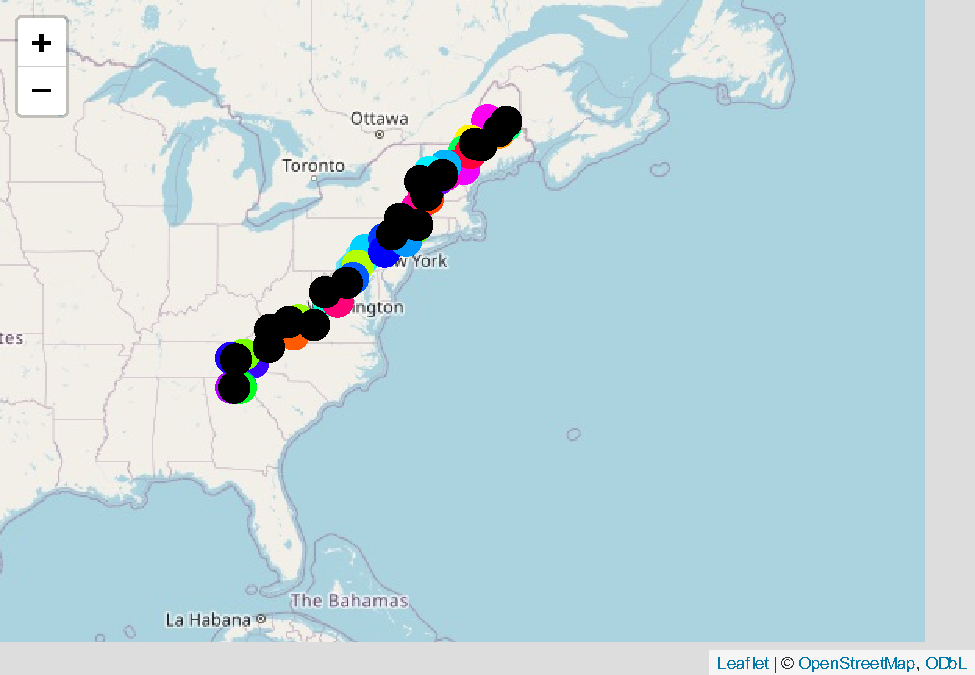
\includegraphics{_main_files/figure-latex/save-centroids-1.pdf}

\begin{Shaded}
\begin{Highlighting}[]
\FunctionTok{saveRDS}\NormalTok{(section\_centroids, }\AttributeTok{file =} \FunctionTok{paste0}\NormalTok{(save\_location, }\StringTok{"section\_centroids.rds"}\NormalTok{))}
\FunctionTok{saveRDS}\NormalTok{(subsection\_centroids, }\AttributeTok{file =} \FunctionTok{paste0}\NormalTok{(save\_location, }\StringTok{"subsection\_centroids.rds"}\NormalTok{))}
\end{Highlighting}
\end{Shaded}

A centroid file was in original repo - but not sure how it was created - took a stab here. Check map above to see if method was acceptable.

\hypertarget{save-plot-attributes}{%
\subsection{Save plot attributes}\label{save-plot-attributes}}

\begin{Shaded}
\begin{Highlighting}[]
\CommentTok{\# create list of abbreviated subsection to append to plot attributes table}
\NormalTok{sub\_attributes\_for\_plots }\OtherTok{\textless{}{-}}\NormalTok{ subsection\_attributes }\SpecialCharTok{\%\textgreater{}\%}
  \FunctionTok{select}\NormalTok{(ECOSUBCD, PROVINCE, SECTION, DOMAIN\_NAM, DIVISION\_N, PROVINCE\_N,}
\NormalTok{         SECTION\_NA, SUBSECTI\_1,ATIntersec,}
\NormalTok{         SUBSECT\_ABBR, SUBSECT\_ABBR\_ST, states)}

\DocumentationTok{\#\# Plot attributes unique locations  }
\NormalTok{plot\_attributes\_final }\OtherTok{\textless{}{-}}\NormalTok{ plot\_attributes }\SpecialCharTok{|\textgreater{}}
  \FunctionTok{right\_join}\NormalTok{(sub\_attributes\_for\_plots, }\AttributeTok{by =} \FunctionTok{join\_by}\NormalTok{(ECOSUBCD)) }\SpecialCharTok{|\textgreater{}}
  \FunctionTok{select}\NormalTok{(}\SpecialCharTok{{-}}\NormalTok{STATECD) }

\DocumentationTok{\#\# Plot attributes by year}
\NormalTok{plot\_attributes\_drop\_geom }\OtherTok{\textless{}{-}}\NormalTok{ plot\_attributes\_final }\SpecialCharTok{|\textgreater{}}
\NormalTok{  sf}\SpecialCharTok{::}\FunctionTok{st\_drop\_geometry}\NormalTok{()}
\NormalTok{plot\_attributes\_by\_year\_final }\OtherTok{\textless{}{-}}\NormalTok{ tpa\_plots\_by\_year }\SpecialCharTok{|\textgreater{}}
  \FunctionTok{select}\NormalTok{(YEAR, pltID) }\SpecialCharTok{|\textgreater{}}
  \FunctionTok{left\_join}\NormalTok{(plot\_attributes\_drop\_geom, }\AttributeTok{by =} \FunctionTok{join\_by}\NormalTok{(pltID))}

\FunctionTok{saveRDS}\NormalTok{(plot\_attributes\_final, }\AttributeTok{file =} \FunctionTok{paste0}\NormalTok{(save\_location, }\StringTok{"plot\_attributes\_locations.rds"}\NormalTok{)) }
\FunctionTok{saveRDS}\NormalTok{(plot\_attributes\_by\_year\_final, }\AttributeTok{file =} \FunctionTok{paste0}\NormalTok{(save\_location, }\StringTok{"plot\_attributes\_by\_year.rds"}\NormalTok{)) }
\end{Highlighting}
\end{Shaded}

\hypertarget{join-subsection-attributes-to-eco}{%
\subsubsection{join subsection attributes to eco}\label{join-subsection-attributes-to-eco}}

\begin{Shaded}
\begin{Highlighting}[]
\NormalTok{eco\_final }\OtherTok{\textless{}{-}}\NormalTok{ eco }\SpecialCharTok{|\textgreater{}}
  \FunctionTok{left\_join}\NormalTok{(subsection\_attributes)}

\FunctionTok{saveRDS}\NormalTok{(eco\_final, }\AttributeTok{file =} \FunctionTok{paste0}\NormalTok{(save\_location, }\StringTok{"eco.rds"}\NormalTok{)) }
\end{Highlighting}
\end{Shaded}

\hypertarget{check-plot-attributes-final}{%
\section{Check plot attributes final}\label{check-plot-attributes-final}}

Note the new Ecosubsection names and ability to detect subsections without FIA plots

\begin{Shaded}
\begin{Highlighting}[]
\CommentTok{\# Visualize plot distance x elevation with plot\_attributes\_final}
\NormalTok{plot\_attributes\_final\_graph }\OtherTok{\textless{}{-}} \FunctionTok{na.omit}\NormalTok{(plot\_attributes\_final)}

\NormalTok{plots\_na }\OtherTok{\textless{}{-}}\NormalTok{ plot\_attributes\_final }\SpecialCharTok{|\textgreater{}}
  \FunctionTok{filter}\NormalTok{(}\FunctionTok{is.na}\NormalTok{(pltID)) }\SpecialCharTok{|\textgreater{}}
  \FunctionTok{pull}\NormalTok{(SUBSECT\_ABBR)}
\NormalTok{plots\_na }\OtherTok{\textless{}{-}} \FunctionTok{paste}\NormalTok{(}\StringTok{"Subsections without plot data:"}\NormalTok{, }\FunctionTok{paste}\NormalTok{(plots\_na, }\AttributeTok{collapse =} \StringTok{", "}\NormalTok{))}

\NormalTok{plot\_attributes\_final\_graph }\SpecialCharTok{|\textgreater{}}
  \FunctionTok{group\_by}\NormalTok{(ECOSUBCD)}\SpecialCharTok{|\textgreater{}}
  \FunctionTok{mutate}\NormalTok{(}\AttributeTok{median\_dist =} \FunctionTok{median}\NormalTok{(distance\_m)) }\SpecialCharTok{|\textgreater{}}
  \FunctionTok{mutate}\NormalTok{(}\AttributeTok{median\_elev =} \FunctionTok{median}\NormalTok{(ELEV)) }\SpecialCharTok{|\textgreater{}}
  \FunctionTok{ggplot}\NormalTok{(}\FunctionTok{aes}\NormalTok{(}\AttributeTok{x=} \FunctionTok{fct\_reorder}\NormalTok{(SUBSECT\_ABBR\_ST, distance\_m), }
             \AttributeTok{y=}\NormalTok{ELEV, }
             \AttributeTok{fill =} \FunctionTok{as.factor}\NormalTok{(median\_elev))) }\SpecialCharTok{+}
  \FunctionTok{geom\_boxplot}\NormalTok{() }\SpecialCharTok{+}
  \FunctionTok{theme}\NormalTok{(}\AttributeTok{axis.text.x =} \FunctionTok{element\_text}\NormalTok{(}\AttributeTok{angle =} \DecValTok{90}\NormalTok{, }\AttributeTok{vjust =} \FloatTok{0.5}\NormalTok{, }\AttributeTok{hjust=}\DecValTok{1}\NormalTok{),}
        \AttributeTok{legend.position =} \StringTok{\textquotesingle{}none\textquotesingle{}}\NormalTok{) }\SpecialCharTok{+}
  \FunctionTok{xlab}\NormalTok{(}\StringTok{"Ecosubsection (from SW to NE)"}\NormalTok{) }\SpecialCharTok{+} \FunctionTok{ylab}\NormalTok{(}\StringTok{"Plot Elevation"}\NormalTok{) }\SpecialCharTok{+}
  \FunctionTok{labs}\NormalTok{(}\AttributeTok{caption =}\NormalTok{ plots\_na)}
\end{Highlighting}
\end{Shaded}

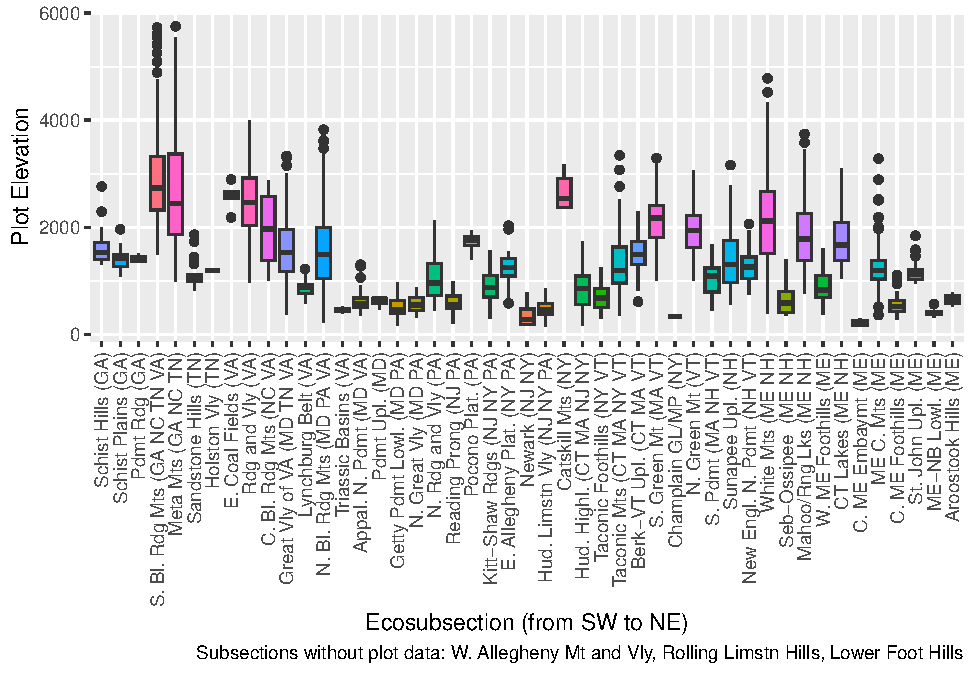
\includegraphics{_main_files/figure-latex/viz-plot-attributes-final-1.pdf}
\#\# Vizualize plots per year

\begin{Shaded}
\begin{Highlighting}[]
\CommentTok{\# Visualize number of plots per subsection per year}
\NormalTok{n\_plots\_per\_year }\OtherTok{\textless{}{-}}\NormalTok{ tpa\_plots }\SpecialCharTok{|\textgreater{}}
\NormalTok{  sf}\SpecialCharTok{::}\FunctionTok{st\_drop\_geometry}\NormalTok{() }\SpecialCharTok{|\textgreater{}}
  \FunctionTok{group\_by}\NormalTok{(ECOSUBCD, YEAR) }\SpecialCharTok{|\textgreater{}}
  \FunctionTok{summarize}\NormalTok{(}\AttributeTok{n\_plots\_per\_year =} \FunctionTok{n}\NormalTok{(), }\AttributeTok{.groups =} \StringTok{\textquotesingle{}drop\textquotesingle{}}\NormalTok{) }\SpecialCharTok{|\textgreater{}}
  \FunctionTok{right\_join}\NormalTok{(subsection\_attributes, }\AttributeTok{by =} \FunctionTok{join\_by}\NormalTok{(ECOSUBCD))}

\NormalTok{n\_plots\_per\_year\_graph }\OtherTok{\textless{}{-}} \FunctionTok{na.omit}\NormalTok{(n\_plots\_per\_year)}

\NormalTok{n\_plots\_per\_year\_graph }\SpecialCharTok{\%\textgreater{}\%}
  \FunctionTok{mutate}\NormalTok{(}\AttributeTok{highlight =} \FunctionTok{case\_when}\NormalTok{(n\_plots\_per\_year }\SpecialCharTok{==} \DecValTok{1} \SpecialCharTok{\textasciitilde{}} \StringTok{"1 plot"}\NormalTok{,}
\NormalTok{                               n\_plots\_per\_year }\SpecialCharTok{==} \DecValTok{2} \SpecialCharTok{\textasciitilde{}} \StringTok{"2 plots"}\NormalTok{,}
                               \AttributeTok{.default =} \ConstantTok{NA}\NormalTok{)) }\SpecialCharTok{\%\textgreater{}\%}
  \FunctionTok{ggplot}\NormalTok{(}\FunctionTok{aes}\NormalTok{(}\AttributeTok{x=}\NormalTok{forcats}\SpecialCharTok{::}\FunctionTok{fct\_reorder}\NormalTok{(SUBSECT\_ABBR\_ST, median\_distance), }
             \AttributeTok{y=}\NormalTok{YEAR, }
             \AttributeTok{size =}\NormalTok{ n\_plots\_per\_year, }
             \AttributeTok{color =}\NormalTok{ highlight)) }\SpecialCharTok{+}
  \FunctionTok{geom\_count}\NormalTok{() }\SpecialCharTok{+}
  \FunctionTok{theme}\NormalTok{(}\AttributeTok{axis.text.x =} \FunctionTok{element\_text}\NormalTok{(}\AttributeTok{angle =} \DecValTok{90}\NormalTok{, }\AttributeTok{vjust =} \FloatTok{0.5}\NormalTok{, }\AttributeTok{hjust=}\DecValTok{1}\NormalTok{)) }\SpecialCharTok{+}
  \FunctionTok{scale\_size\_area}\NormalTok{() }\SpecialCharTok{+}
  \FunctionTok{scale\_color\_manual}\NormalTok{(}\AttributeTok{values =} \FunctionTok{c}\NormalTok{(}\StringTok{"red2"}\NormalTok{, }\StringTok{"cyan3"}\NormalTok{, }\StringTok{"grey50"}\NormalTok{),}
                     \AttributeTok{breaks =} \FunctionTok{c}\NormalTok{(}\StringTok{"1 plot"}\NormalTok{, }\StringTok{"2 plots"}\NormalTok{)) }\SpecialCharTok{+}
  \FunctionTok{xlab}\NormalTok{(}\StringTok{"Ecosubsection (from SW to NE)"}\NormalTok{) }\SpecialCharTok{+}
  \FunctionTok{labs}\NormalTok{(}\AttributeTok{caption =}\NormalTok{ plots\_na)}
\end{Highlighting}
\end{Shaded}

\hypertarget{make}{%
\chapter{Make}\label{make}}

\hypertarget{load-data}{%
\section{Load data}\label{load-data}}

Location where data was saved from previous chapter (clip)

\begin{Shaded}
\begin{Highlighting}[]
\DocumentationTok{\#\# default location:}
\NormalTok{load\_location\_default }\OtherTok{\textless{}{-}} \StringTok{\textquotesingle{}./clip\_FIA/\textquotesingle{}}
\DocumentationTok{\#\# custom location:}
\NormalTok{load\_location\_custom }\OtherTok{\textless{}{-}} \StringTok{\textquotesingle{}C:/Users/JJGross/Documents/R\_projects/FIA\_data/clip\_FIA/\textquotesingle{}} 
\CommentTok{\#set variable}
\NormalTok{load\_location }\OtherTok{\textless{}{-}}\NormalTok{ load\_location\_custom}
\end{Highlighting}
\end{Shaded}

Load data and set as default argument variables

\begin{Shaded}
\begin{Highlighting}[]
\DocumentationTok{\#\# Load most recent (MR) Appalachian trail (at) dataset:}
\NormalTok{at\_MR }\OtherTok{\textless{}{-}} \FunctionTok{read\_rds}\NormalTok{(}\AttributeTok{file =} \FunctionTok{paste0}\NormalTok{(load\_location, }\StringTok{"at\_FIA\_MR.rds"}\NormalTok{))}
\DocumentationTok{\#\# Load entire Appalachian trail (at) dataset:}
\NormalTok{at }\OtherTok{\textless{}{-}} \FunctionTok{read\_rds}\NormalTok{(}\AttributeTok{file =} \FunctionTok{paste0}\NormalTok{(load\_location, }\StringTok{"at\_FIA.rds"}\NormalTok{)) }
\DocumentationTok{\#\# Load eco}
\NormalTok{eco }\OtherTok{\textless{}{-}} \FunctionTok{read\_rds}\NormalTok{(}\AttributeTok{file =} \FunctionTok{paste0}\NormalTok{(load\_location, }\StringTok{"eco.rds"}\NormalTok{)) }

\DocumentationTok{\#\# Set default variables for rFIA function:}
\NormalTok{database\_variable }\OtherTok{\textless{}{-}}\NormalTok{ at}
\NormalTok{polys\_variable }\OtherTok{\textless{}{-}}\NormalTok{ eco}
\end{Highlighting}
\end{Shaded}

\hypertarget{save-location-1}{%
\section{Save location}\label{save-location-1}}

Choose where final tables will be saved:

\begin{Shaded}
\begin{Highlighting}[]
\DocumentationTok{\#\# default location:}
\NormalTok{save\_default }\OtherTok{\textless{}{-}} \StringTok{\textquotesingle{}./summary\_data/\textquotesingle{}} 
\DocumentationTok{\#\# Alternatively, enter specific custom location:}
\NormalTok{save\_custom }\OtherTok{\textless{}{-}} \StringTok{\textquotesingle{}C:/Users/JJGross/Documents/R\_projects/FIA\_data/summary\_data/\textquotesingle{}}

\NormalTok{save\_location }\OtherTok{\textless{}{-}}\NormalTok{ save\_custom}

\DocumentationTok{\#\# Create directory if it doesn\textquotesingle{}t already exist}
\ControlFlowTok{if}\NormalTok{ (}\SpecialCharTok{!}\FunctionTok{dir.exists}\NormalTok{(save\_location)) \{}\FunctionTok{dir.create}\NormalTok{(save\_location)\}}
\end{Highlighting}
\end{Shaded}

\hypertarget{metrics}{%
\section{Metrics}\label{metrics}}

Derive population estimates (at the plot- or the ecoregion-scale) for each forest health metric:

\textbf{Live tree abundance}

\begin{itemize}
\tightlist
\item
  \protect\hyperlink{tpa}{tpa}
\item
  \protect\hyperlink{tpa_spp}{tpa\_spp}
\item
  \protect\hyperlink{tpa_spp_sizecl}{tpa\_spp\_sizecl}
\item
  \protect\hyperlink{biomass}{biomass}
\end{itemize}

\textbf{Species diversity of live trees}

\begin{itemize}
\tightlist
\item
  \protect\hyperlink{diversity}{diversity}
\end{itemize}

\textbf{Tree vital rates}

\begin{itemize}
\tightlist
\item
  \protect\hyperlink{growth}{growth}
\end{itemize}

\textbf{Forest demographic rates}

\begin{itemize}
\tightlist
\item
  \protect\hyperlink{mortality}{mortality}
\end{itemize}

\textbf{Regeneration abundance}

\begin{itemize}
\tightlist
\item
  \protect\hyperlink{seedlings}{seedlings}
\item
  \protect\hyperlink{seedlings_spp}{seedlings\_spp}
\item
  \protect\hyperlink{saplings}{saplings}
\item
  \protect\hyperlink{saplings_spp}{saplings\_spp}
\item
  \protect\hyperlink{saplings_sizecl}{saplings\_sizecl}
\end{itemize}

\textbf{Snags}

\begin{itemize}
\tightlist
\item
  \protect\hyperlink{snag_abundance}{snag\_abundance}
\item
  \protect\hyperlink{dead_and_live_tpa}{dead\_and\_live\_tpa}
\item
  \protect\hyperlink{snag_volume}{snag\_volume}
\end{itemize}

\textbf{Down woody material}

\begin{itemize}
\tightlist
\item
  \protect\hyperlink{downwoody}{downwoody}
\end{itemize}

\textbf{Invasive plant abundance}

\begin{itemize}
\tightlist
\item
  \protect\hyperlink{invasive}{invasive}
\end{itemize}

\textbf{Stand structural stage distributions}

\begin{itemize}
\tightlist
\item
  \protect\hyperlink{ss}{ss}
\end{itemize}

Each of the following subsections illustrates how to use the variety of functions in \texttt{rFIA} to calculate these metrics.

\hypertarget{argument-variables}{%
\subsection{Argument Variables}\label{argument-variables}}

Are plot-level records desired within each \texttt{SUBSECTION}? If so, run the entire \texttt{03-make.Rmd} with \texttt{by\_plot\_variable} set to \texttt{TRUE}. Otherwise, leave \texttt{by\_plot\_variable\ \textless{}-\ FALSE} to aggregate FIA plots at \texttt{SUBSECTION} level.

\begin{itemize}
\tightlist
\item
  \texttt{by\_plot\_variable\ \textless{}-\ FALSE} means tables are summarized at SUBSECTION-level
\item
  \texttt{by\_plot\_variable\ \textless{}-\ TRUE} means tables are summarized at the FIA plot-level
\end{itemize}

\begin{Shaded}
\begin{Highlighting}[]
\NormalTok{by\_plot\_variable }\OtherTok{\textless{}{-}} \ConstantTok{FALSE}
\end{Highlighting}
\end{Shaded}

\begin{itemize}
\tightlist
\item
  \texttt{most\_recent\ \textless{}-\ FALSE} means all FIA plots are included in the data tables
\item
  \texttt{most\_recent\ \textless{}-\ TRUE} means only the most recent FIA plots are included
\end{itemize}

\begin{Shaded}
\begin{Highlighting}[]
\NormalTok{most\_recent }\OtherTok{\textless{}{-}} \ConstantTok{TRUE}
\end{Highlighting}
\end{Shaded}

The code chunk below automatically updates argument variables and folder save location based on above user input (blue boxes) to \texttt{by\_plot\_variable} and \texttt{most\_recent}. Code chunk also specifies the number of processing cores to use during the execution of rFIA functions. See the rFIA webpage \href{https://rfia.netlify.app/tutorial/bigdata/}{Tips for working with Big Data} for more information.

\begin{Shaded}
\begin{Highlighting}[]
\DocumentationTok{\#\# save tables to new folder if by\_plot\_variable is TRUE}
\ControlFlowTok{if}\NormalTok{ (by\_plot\_variable }\SpecialCharTok{==} \ConstantTok{TRUE}\NormalTok{) \{}
  \CommentTok{\# new save location folder}
  \FunctionTok{ifelse}\NormalTok{(}\SpecialCharTok{!}\FunctionTok{dir.exists}\NormalTok{(}\FunctionTok{file.path}\NormalTok{(save\_location)), }\FunctionTok{dir.create}\NormalTok{(}\FunctionTok{file.path}\NormalTok{(save\_location)), }\ConstantTok{FALSE}\NormalTok{)}
\NormalTok{  save\_location }\OtherTok{\textless{}{-}} \FunctionTok{paste0}\NormalTok{(save\_location, }\StringTok{"by\_plot\_variable/"}\NormalTok{)}
  
\NormalTok{\}}

\DocumentationTok{\#\# if \textquotesingle{}most\_recent == TRUE\textquotesingle{}, than change database\_variable to \textquotesingle{}at\_MR\textquotesingle{} database }
\DocumentationTok{\#\# and create new folder to save MR tables to. }
\ControlFlowTok{if}\NormalTok{ (most\_recent }\SpecialCharTok{==} \ConstantTok{TRUE}\NormalTok{) \{}
\NormalTok{  database\_variable }\OtherTok{\textless{}{-}}\NormalTok{ at\_MR}
  \CommentTok{\# new save location folder}
  \FunctionTok{ifelse}\NormalTok{(}\SpecialCharTok{!}\FunctionTok{dir.exists}\NormalTok{(}\FunctionTok{file.path}\NormalTok{(save\_location, }\StringTok{"most\_recent"}\NormalTok{)), }
         \FunctionTok{dir.create}\NormalTok{(}\FunctionTok{file.path}\NormalTok{(save\_location, }\StringTok{"most\_recent"}\NormalTok{)), }\ConstantTok{FALSE}\NormalTok{)}
\NormalTok{  save\_location }\OtherTok{\textless{}{-}} \FunctionTok{paste0}\NormalTok{(save\_location, }\StringTok{"most\_recent/"}\NormalTok{)}
\NormalTok{\}}

\DocumentationTok{\#\# default number of processing cores to utilize in rFIA function arguments below.}
\NormalTok{cores\_variable }\OtherTok{\textless{}{-}}\NormalTok{ parallel}\SpecialCharTok{::}\FunctionTok{detectCores}\NormalTok{()}\SpecialCharTok{{-}}\DecValTok{2}
\end{Highlighting}
\end{Shaded}

\hypertarget{population-estimate-method}{%
\subsection{Population estimate method}\label{population-estimate-method}}

Functions in \texttt{rFIA} can be used to derive population estimates of forest data using 5 unique estimators (i.e.~different methods for panel combination) using the \texttt{method} argument in each function. For the purposes of forest population estimation for APPA, only the \texttt{method\ =\ ANNUAL} argument is used (i.e.~no panel combination). For more information on panel combinations see the rFIA \href{https://rfia.netlify.app/tutorial/ae/}{Alternative design-based estimators} page.

\begin{Shaded}
\begin{Highlighting}[]
\DocumentationTok{\#\# Set method variable for rFIA function arguments here:}
\NormalTok{method\_variable }\OtherTok{\textless{}{-}} \StringTok{"ANNUAL"}
\end{Highlighting}
\end{Shaded}

Note that when using \texttt{method\ =\ "ANNUAL"} all \texttt{rFIA::} functions result with the following error message:

``Bad stratification, i.e., strata too small to compute variance of annual panels. If you are only interested in totals and/or ratio estimates, disregard this. However, if interested in variance (e.g., for confidence intervals) try using method =''TI''.''

\hypertarget{live-tree-abundance}{%
\section{Live tree abundance}\label{live-tree-abundance}}

The \href{https://rdrr.io/cran/rFIA/man/tpa.html}{rFIA::tpa()} function Produces tree per acre (TPA) and basal area per acre (BAA) estimates from FIA data, along with population totals for each variable. Options to group estimates by species, size class, and other variables defined in the FIADB.

Argument \texttt{treeDomain\ =\ DIA\ \textbackslash{}\textgreater{}=\ 5} results in estimates only utilizing tree diameters above 5 inches DBH.

\hypertarget{tpa}{%
\subsection{tpa}\label{tpa}}

\begin{Shaded}
\begin{Highlighting}[]
\DocumentationTok{\#\# Trees per Acre (species and size classes lumped)}
\NormalTok{tpa }\OtherTok{\textless{}{-}}\NormalTok{ rFIA}\SpecialCharTok{::}\FunctionTok{tpa}\NormalTok{(}
  \AttributeTok{db =}\NormalTok{ database\_variable,}
  \AttributeTok{byPlot =}\NormalTok{ by\_plot\_variable,}
  \AttributeTok{polys =}\NormalTok{ polys\_variable,}
  \AttributeTok{method =}\NormalTok{ method\_variable,}
  \AttributeTok{nCores =}\NormalTok{ cores\_variable,}
  \AttributeTok{returnSpatial =} \ConstantTok{TRUE}\NormalTok{,}
  \AttributeTok{treeType =} \StringTok{"live"}\NormalTok{,}
  \AttributeTok{totals =} \ConstantTok{TRUE}\NormalTok{,}
  \AttributeTok{treeDomain =}\NormalTok{ DIA }\SpecialCharTok{\textgreater{}=} \DecValTok{5}
\NormalTok{) }
\FunctionTok{saveRDS}\NormalTok{(tpa, }\FunctionTok{paste0}\NormalTok{(save\_location, }\StringTok{"tpa.rds"}\NormalTok{))}
\end{Highlighting}
\end{Shaded}

\hypertarget{tpa_spp}{%
\subsection{tpa\_spp}\label{tpa_spp}}

\begin{Shaded}
\begin{Highlighting}[]
\DocumentationTok{\#\# Trees per Acre by species (size{-}classes lumped)}
\NormalTok{tpa\_spp }\OtherTok{\textless{}{-}}\NormalTok{ rFIA}\SpecialCharTok{::}\FunctionTok{tpa}\NormalTok{(}
  \AttributeTok{db =}\NormalTok{ database\_variable,}
  \AttributeTok{byPlot =}\NormalTok{ by\_plot\_variable,}
  \AttributeTok{polys =}\NormalTok{ polys\_variable,}
  \AttributeTok{method =}\NormalTok{ method\_variable,}
  \AttributeTok{nCores =}\NormalTok{ cores\_variable,}
  \AttributeTok{returnSpatial =} \ConstantTok{TRUE}\NormalTok{,}
  \AttributeTok{treeType =} \StringTok{"live"}\NormalTok{,}
  \AttributeTok{totals =} \ConstantTok{TRUE}\NormalTok{,}
  \AttributeTok{treeDomain =}\NormalTok{ DIA }\SpecialCharTok{\textgreater{}=} \DecValTok{5}\NormalTok{,}
  \AttributeTok{bySpecies =} \ConstantTok{TRUE}\NormalTok{,}
  \AttributeTok{bySizeClass =} \ConstantTok{FALSE}
\NormalTok{) }
\FunctionTok{saveRDS}\NormalTok{(tpa\_spp, }\FunctionTok{paste0}\NormalTok{(save\_location, }\StringTok{"tpa\_spp.rds"}\NormalTok{))}
\end{Highlighting}
\end{Shaded}

\hypertarget{tpa_spp_sizecl}{%
\subsection{tpa\_spp\_sizecl}\label{tpa_spp_sizecl}}

\begin{Shaded}
\begin{Highlighting}[]
\DocumentationTok{\#\# Trees per Acre (by species and size{-}class)}
\NormalTok{tpa\_spp\_sizecl }\OtherTok{\textless{}{-}}\NormalTok{ rFIA}\SpecialCharTok{::}\FunctionTok{tpa}\NormalTok{(}
  \AttributeTok{db =}\NormalTok{ database\_variable,}
  \AttributeTok{byPlot =}\NormalTok{ by\_plot\_variable,}
  \AttributeTok{polys =}\NormalTok{ polys\_variable,}
  \AttributeTok{method =}\NormalTok{ method\_variable,}
  \AttributeTok{nCores =}\NormalTok{ cores\_variable,}
  \AttributeTok{returnSpatial =} \ConstantTok{TRUE}\NormalTok{,}
  \AttributeTok{treeType =} \StringTok{"live"}\NormalTok{,}
  \AttributeTok{totals =} \ConstantTok{TRUE}\NormalTok{,}
  \AttributeTok{treeDomain =}\NormalTok{ DIA }\SpecialCharTok{\textgreater{}=} \DecValTok{5}\NormalTok{,}
  \AttributeTok{bySpecies =} \ConstantTok{TRUE}\NormalTok{,}
  \AttributeTok{bySizeClass =} \ConstantTok{TRUE}
\NormalTok{)}
\FunctionTok{saveRDS}\NormalTok{(tpa\_spp\_sizecl, }\FunctionTok{paste0}\NormalTok{(save\_location, }\StringTok{"tpa\_spp\_sizecl.rds"}\NormalTok{))}
\end{Highlighting}
\end{Shaded}

\hypertarget{biomass}{%
\subsection{biomass}\label{biomass}}

The \href{https://rdrr.io/cran/rFIA/man/biomass.html}{rFIA::biomass()} function produces estimates of volume (cu.ft./acre), biomass (tons/acre), and carbon (tons/acre) with options to group estimates by species, size class, and other variables defined in the FIADB.

\begin{Shaded}
\begin{Highlighting}[]
\DocumentationTok{\#\# biomass (by species and size{-}class)}
\CommentTok{\# biomass \textless{}{-} rFIA::biomass(db = database\_variable,}
\CommentTok{\#            byPlot = by\_plot\_variable,}
\CommentTok{\#            polys = polys\_variable, }
\CommentTok{\#            method = method\_variable,}
\CommentTok{\#            nCores = cores\_variable,}
\CommentTok{\#            returnSpatial = TRUE,}
\CommentTok{\#            treeType = "live",}
\CommentTok{\#            totals = TRUE,}
\CommentTok{\#            treeDomain = DIA \textgreater{}= 5,}
\CommentTok{\#            bySpecies = TRUE, }
\CommentTok{\#            bySizeClass = TRUE) }
\CommentTok{\# saveRDS(biomass, paste0(save\_location, "biomass.rds"))}
\end{Highlighting}
\end{Shaded}

Note that the \texttt{rFIA::biomass()} function currently produces the following error and needs attention from package developers.

Error in fcase(is.na(DIA), NA\_real\_, !is.na(DRYBIO\_WDLD\_SPP), DRYBIO\_WDLD\_SPP/(jTotal - : object `DRYBIO\_WDLD\_SPP' not found

\hypertarget{species-diversity-of-live-trees}{%
\section{Species diversity of live trees}\label{species-diversity-of-live-trees}}

The \href{https://rdrr.io/cran/rFIA/man/diversity.html}{rFIA::diversity()} function produces estimates of diversity from FIA data. Returns Shannon's Index (H), Shannon's Equitability (Eh), and Richness (S) for alpha (mean/SE of stands), beta, and gamma diversity. Default behavior estimates species diversity, using TPA as a state variable and Species Code (SPCD) to groups of individuals.

\hypertarget{diversity}{%
\subsection{diversity}\label{diversity}}

\begin{Shaded}
\begin{Highlighting}[]
\DocumentationTok{\#\# Diversity}
\NormalTok{diversity }\OtherTok{\textless{}{-}}\NormalTok{ rFIA}\SpecialCharTok{::}\FunctionTok{diversity}\NormalTok{(}
  \AttributeTok{db =}\NormalTok{ database\_variable,}
  \AttributeTok{byPlot =}\NormalTok{ by\_plot\_variable,}
  \AttributeTok{polys =}\NormalTok{ polys\_variable,}
  \AttributeTok{method =}\NormalTok{ method\_variable,}
  \AttributeTok{nCores =}\NormalTok{ cores\_variable,}
  \AttributeTok{returnSpatial =} \ConstantTok{TRUE}\NormalTok{,}
  \AttributeTok{treeType =} \StringTok{"live"}\NormalTok{,}
  \AttributeTok{totals =} \ConstantTok{TRUE}\NormalTok{,}
  \AttributeTok{treeDomain =}\NormalTok{ DIA }\SpecialCharTok{\textgreater{}=} \DecValTok{5}
\NormalTok{)}
\FunctionTok{saveRDS}\NormalTok{(diversity, }\FunctionTok{paste0}\NormalTok{(save\_location, }\StringTok{"diversity.rds"}\NormalTok{))}
\end{Highlighting}
\end{Shaded}

\hypertarget{tree-growth-rates}{%
\section{Tree growth rates}\label{tree-growth-rates}}

The \href{https://rdrr.io/cran/rFIA/man/vitalRates.html}{rFIA::vitalRates()} function computes estimates of average annual DBH (inches/ yr), basal area (sq. ft./ yr), biomass (short tons/ yr), and net volume (cu. ft./yr) growth rates for individual stems, along with average annual basal area and net volume growth per acre.

To calcuate by size class include argument \texttt{bySizeClass\ =TRUE}

To estimate net growth rates (include trees that have recruited or died in estimates), use \texttt{treeType\ =\ \textquotesingle{}all\textquotesingle{}} (default)

To exclude stems that died or recruited into the population between plot measurements set \texttt{treeType\ =\ \textquotesingle{}live\textquotesingle{}}

\hypertarget{growth}{%
\subsection{growth}\label{growth}}

\begin{Shaded}
\begin{Highlighting}[]
\DocumentationTok{\#\# Tree DBH growth}
\NormalTok{growth }\OtherTok{\textless{}{-}}\NormalTok{ rFIA}\SpecialCharTok{::}\FunctionTok{vitalRates}\NormalTok{(}
  \AttributeTok{db =}\NormalTok{ database\_variable,}
  \AttributeTok{byPlot =}\NormalTok{ by\_plot\_variable,}
  \AttributeTok{polys =}\NormalTok{ polys\_variable,}
  \AttributeTok{method =}\NormalTok{ method\_variable,}
  \AttributeTok{nCores =}\NormalTok{ cores\_variable,}
  \AttributeTok{returnSpatial =} \ConstantTok{TRUE}\NormalTok{,}
  \AttributeTok{treeType =} \StringTok{"live"}\NormalTok{,}
  \AttributeTok{totals =} \ConstantTok{TRUE}\NormalTok{,}
  \AttributeTok{treeDomain =}\NormalTok{ DIA }\SpecialCharTok{\textgreater{}=} \DecValTok{5}\NormalTok{,}
  \AttributeTok{bySpecies =} \ConstantTok{TRUE}\NormalTok{,}
  \AttributeTok{variance =} \ConstantTok{TRUE} \CommentTok{\# note error message: "Bad stratification, i.e., strata too small to compute variance of annual panels." }
\NormalTok{)}
\FunctionTok{saveRDS}\NormalTok{(growth, }\FunctionTok{paste0}\NormalTok{(save\_location, }\StringTok{"growth.rds"}\NormalTok{))}
\end{Highlighting}
\end{Shaded}

\hypertarget{forest-demographic-rates}{%
\section{Forest demographic rates}\label{forest-demographic-rates}}

The \href{https://rdrr.io/cran/rFIA/man/growMort.html}{rFIA::growMort()} function estimates of annual growth, recruitment, natural mortality, and harvest rates, along with population estimates for each variable.

Recruitment events are defined as when a live stem which is less than 5 inches DBH at time 1, grows to or beyond 5 inches DBH by time 2. This does NOT include stems which grow beyond the 5-inch diameter criteria and are then subject to mortality prior to remeasurement. Natural mortality is defined as when a live stem is subject to non-harvest mortality between successive measurement periods. Finally, harvest is defined as when a live stem is cut and removed between successive measurements.

\hypertarget{mortality}{%
\subsection{mortality}\label{mortality}}

To estimate mortality per species:

\begin{Shaded}
\begin{Highlighting}[]
\DocumentationTok{\#\# mortality}
\NormalTok{mortality }\OtherTok{\textless{}{-}}\NormalTok{ rFIA}\SpecialCharTok{::}\FunctionTok{growMort}\NormalTok{(}
  \AttributeTok{db =}\NormalTok{ database\_variable,}
  \AttributeTok{byPlot =}\NormalTok{ by\_plot\_variable,}
  \AttributeTok{polys =}\NormalTok{ polys\_variable,}
  \AttributeTok{method =}\NormalTok{ method\_variable,}
  \AttributeTok{nCores =}\NormalTok{ cores\_variable,}
  \AttributeTok{returnSpatial =} \ConstantTok{TRUE}\NormalTok{,}
  \AttributeTok{treeType =} \StringTok{"all"}\NormalTok{, }\CommentTok{\#default, includes all stems, live and dead}
  \AttributeTok{totals =} \ConstantTok{TRUE}\NormalTok{,}
  \AttributeTok{treeDomain =}\NormalTok{ DIA }\SpecialCharTok{\textgreater{}=} \DecValTok{5}\NormalTok{,}
  \AttributeTok{bySpecies =} \ConstantTok{TRUE}\NormalTok{,}
  \AttributeTok{variance =} \ConstantTok{TRUE} \CommentTok{\# note error message: "Bad stratification, i.e., strata too small to compute variance of annual panels." }
\NormalTok{)}
\FunctionTok{saveRDS}\NormalTok{(mortality, }\FunctionTok{paste0}\NormalTok{(save\_location, }\StringTok{"mortality.rds"}\NormalTok{))}
\end{Highlighting}
\end{Shaded}

Column \texttt{mortality\$MORT\_PERC} results in \texttt{Inf} for each row. Suspected error with \texttt{rFIA::growMort()} because none of the tables produced had any values in \texttt{MORT\_PREC}

\hypertarget{regeneration-abundance}{%
\section{Regeneration abundance}\label{regeneration-abundance}}

The \href{https://rdrr.io/cran/rFIA/man/seedling.html}{rFIA::seedlings()} and \href{https://rdrr.io/cran/rFIA/man/tpa.html}{rFIA::tpa()} functions are used to estimate regeneration of seedlings and sapling, respectively. Note that querying saplings can be achieved within the \texttt{rFIA::tpa()} function by setting the tree domain argument \texttt{treeDomain\ =\ DIA\ \textless{}\ 5}. Stems below 1 inch DBH are not included in output of \texttt{rFIA::tpa()} because FIA seedlings (\textless1 inch DBH) are sampled differently and therefore queried using the distinct \texttt{rFIA::seedlings()} function.

\hypertarget{seedlings}{%
\subsection{seedlings}\label{seedlings}}

Seedling abundance (trees per acre) is computed using the distinct \texttt{rFIA::seedlings()} function, not the \texttt{rFIA::tpa()} function.

The \href{https://www.fs.usda.gov/research/understory/forest-inventory-and-analysis-glossary-standard-terminology}{FIA glossary} defines seedlings as: ``Live trees smaller than 1.0 inch (2.5 cm) d.b.h./d.r.c. that are at least 6 inches (15.2 cm) in height for softwoods and 12-inches (30.5 cm) in height for hardwoods.''

\begin{Shaded}
\begin{Highlighting}[]
\DocumentationTok{\#\# Trees per acre of seedlings (\textless{}1 inch DBH)}
\NormalTok{seedlings }\OtherTok{\textless{}{-}}\NormalTok{ rFIA}\SpecialCharTok{::}\FunctionTok{seedling}\NormalTok{(}
  \AttributeTok{db =}\NormalTok{ database\_variable,}
  \AttributeTok{byPlot =}\NormalTok{ by\_plot\_variable,}
  \AttributeTok{polys =}\NormalTok{ polys\_variable,}
  \AttributeTok{method =}\NormalTok{ method\_variable,}
  \AttributeTok{nCores =}\NormalTok{ cores\_variable,}
  \AttributeTok{returnSpatial =} \ConstantTok{TRUE}\NormalTok{,}
  \AttributeTok{totals =} \ConstantTok{TRUE}
\NormalTok{) }
\FunctionTok{saveRDS}\NormalTok{(seedlings, }\FunctionTok{paste0}\NormalTok{(save\_location, }\StringTok{"seedlings.rds"}\NormalTok{))}
\end{Highlighting}
\end{Shaded}

\hypertarget{seedlings_spp}{%
\subsection{seedlings\_spp}\label{seedlings_spp}}

\begin{Shaded}
\begin{Highlighting}[]
\DocumentationTok{\#\# Trees per acre of seedlings by species}
\NormalTok{seedlings\_spp }\OtherTok{\textless{}{-}}\NormalTok{ rFIA}\SpecialCharTok{::}\FunctionTok{seedling}\NormalTok{(}
  \AttributeTok{db =}\NormalTok{ database\_variable,}
  \AttributeTok{byPlot =}\NormalTok{ by\_plot\_variable,}
  \AttributeTok{polys =}\NormalTok{ polys\_variable,}
  \AttributeTok{method =}\NormalTok{ method\_variable,}
  \AttributeTok{nCores =}\NormalTok{ cores\_variable,}
  \AttributeTok{returnSpatial =} \ConstantTok{TRUE}\NormalTok{,}
  \AttributeTok{totals =} \ConstantTok{TRUE}\NormalTok{,}
  \AttributeTok{bySpecies =} \ConstantTok{TRUE} \CommentTok{\# by species}
\NormalTok{) }
\FunctionTok{saveRDS}\NormalTok{(seedlings\_spp, }\FunctionTok{paste0}\NormalTok{(save\_location, }\StringTok{"seedlings\_spp.rds"}\NormalTok{))}
\end{Highlighting}
\end{Shaded}

\hypertarget{saplings}{%
\subsection{saplings}\label{saplings}}

Saplings must use \texttt{rFIA::tpa()} function with \texttt{treeDomain\ =\ DIA\ \textless{}\ 5} argument To estimate sapling size class (1 to 4.9 inch DBH).

\begin{Shaded}
\begin{Highlighting}[]
\DocumentationTok{\#\# Trees per acre of saplings (trees greater than 1 inch DBH, and less than 5 inch DBH)}
\NormalTok{saplings }\OtherTok{\textless{}{-}}\NormalTok{ rFIA}\SpecialCharTok{::}\FunctionTok{tpa}\NormalTok{(}
  \AttributeTok{db =}\NormalTok{ database\_variable,}
  \AttributeTok{byPlot =}\NormalTok{ by\_plot\_variable,}
  \AttributeTok{polys =}\NormalTok{ polys\_variable,}
  \AttributeTok{method =}\NormalTok{ method\_variable,}
  \AttributeTok{nCores =}\NormalTok{ cores\_variable,}
  \AttributeTok{returnSpatial =} \ConstantTok{TRUE}\NormalTok{,}
  \AttributeTok{treeType =} \StringTok{"live"}\NormalTok{,}
  \AttributeTok{totals =} \ConstantTok{TRUE}\NormalTok{,}
  \AttributeTok{treeDomain =}\NormalTok{ DIA }\SpecialCharTok{\textless{}} \DecValTok{5}
\NormalTok{) }
\FunctionTok{saveRDS}\NormalTok{(saplings, }\FunctionTok{paste0}\NormalTok{(save\_location, }\StringTok{"saplings.rds"}\NormalTok{))}
\end{Highlighting}
\end{Shaded}

\hypertarget{saplings_spp}{%
\subsection{saplings\_spp}\label{saplings_spp}}

\begin{Shaded}
\begin{Highlighting}[]
\DocumentationTok{\#\# Trees per acre of saplings by species }
\NormalTok{saplings\_spp }\OtherTok{\textless{}{-}}\NormalTok{ rFIA}\SpecialCharTok{::}\FunctionTok{tpa}\NormalTok{(}
  \AttributeTok{db =}\NormalTok{ database\_variable,}
  \AttributeTok{byPlot =}\NormalTok{ by\_plot\_variable,}
  \AttributeTok{polys =}\NormalTok{ polys\_variable,}
  \AttributeTok{method =}\NormalTok{ method\_variable,}
  \AttributeTok{nCores =}\NormalTok{ cores\_variable,}
  \AttributeTok{returnSpatial =} \ConstantTok{TRUE}\NormalTok{,}
  \AttributeTok{treeType =} \StringTok{"live"}\NormalTok{,}
  \AttributeTok{totals =} \ConstantTok{TRUE}\NormalTok{,}
  \AttributeTok{treeDomain =}\NormalTok{ DIA }\SpecialCharTok{\textless{}} \DecValTok{5}\NormalTok{,}
  \AttributeTok{bySpecies =} \ConstantTok{TRUE}\NormalTok{, }\CommentTok{\# by species}
  \AttributeTok{bySizeClass =} \ConstantTok{FALSE}
\NormalTok{) }
\FunctionTok{saveRDS}\NormalTok{(saplings\_spp, }\FunctionTok{paste0}\NormalTok{(save\_location, }\StringTok{"saplings\_spp.rds"}\NormalTok{))}
\end{Highlighting}
\end{Shaded}

\hypertarget{saplings_sizecl}{%
\subsection{saplings\_sizecl}\label{saplings_sizecl}}

\begin{Shaded}
\begin{Highlighting}[]
\DocumentationTok{\#\# Trees per acre of saplings by size class }
\NormalTok{saplings\_sizecl }\OtherTok{\textless{}{-}}\NormalTok{ rFIA}\SpecialCharTok{::}\FunctionTok{tpa}\NormalTok{(}
  \AttributeTok{db =}\NormalTok{ database\_variable,}
  \AttributeTok{byPlot =}\NormalTok{ by\_plot\_variable,}
  \AttributeTok{polys =}\NormalTok{ polys\_variable,}
  \AttributeTok{method =}\NormalTok{ method\_variable,}
  \AttributeTok{nCores =}\NormalTok{ cores\_variable,}
  \AttributeTok{returnSpatial =} \ConstantTok{TRUE}\NormalTok{,}
  \AttributeTok{treeType =} \StringTok{"live"}\NormalTok{,}
  \AttributeTok{totals =} \ConstantTok{TRUE}\NormalTok{,}
  \AttributeTok{treeDomain =}\NormalTok{ DIA }\SpecialCharTok{\textless{}} \DecValTok{5}\NormalTok{,}
  \AttributeTok{bySpecies =} \ConstantTok{FALSE}\NormalTok{,}
  \AttributeTok{bySizeClass =} \ConstantTok{TRUE} \CommentTok{\# by size class}
\NormalTok{) }
\FunctionTok{saveRDS}\NormalTok{(saplings\_sizecl, }\FunctionTok{paste0}\NormalTok{(save\_location, }\StringTok{"saplings\_sizecl.rds"}\NormalTok{))}
\end{Highlighting}
\end{Shaded}

\hypertarget{snags}{%
\section{Snags}\label{snags}}

\href{https://rdrr.io/cran/rFIA/man/tpa.html}{rFIA::tpa()} and \href{https://rdrr.io/cran/rFIA/man/biomass.html}{rFIA::biomass()} can be used to estimate snag abundance, volume, and percentage.

\hypertarget{snag_abundance}{%
\subsection{snag\_abundance}\label{snag_abundance}}

\texttt{treeType\ =\ "dead"} \texttt{bySizeClass\ =\ TRUE}

\begin{Shaded}
\begin{Highlighting}[]
\DocumentationTok{\#\# Snags per acre}
\NormalTok{snag\_abundance }\OtherTok{\textless{}{-}}\NormalTok{ rFIA}\SpecialCharTok{::}\FunctionTok{tpa}\NormalTok{(}
  \AttributeTok{db =}\NormalTok{ database\_variable,}
  \AttributeTok{byPlot =}\NormalTok{ by\_plot\_variable,}
  \AttributeTok{polys =}\NormalTok{ polys\_variable,}
  \AttributeTok{method =}\NormalTok{ method\_variable,}
  \AttributeTok{nCores =}\NormalTok{ cores\_variable,}
  \AttributeTok{returnSpatial =} \ConstantTok{TRUE}\NormalTok{,}
  \AttributeTok{treeType =} \StringTok{"dead"}\NormalTok{,}
  \AttributeTok{totals =} \ConstantTok{TRUE}\NormalTok{,}
  \AttributeTok{treeDomain =}\NormalTok{ DIA }\SpecialCharTok{\textgreater{}=} \DecValTok{5}\NormalTok{,}
  \AttributeTok{bySizeClass =} \ConstantTok{TRUE}
\NormalTok{)}

\FunctionTok{saveRDS}\NormalTok{(snag\_abundance, }\FunctionTok{paste0}\NormalTok{(save\_location, }\StringTok{"snag\_abundance.rds"}\NormalTok{))}
\end{Highlighting}
\end{Shaded}

\hypertarget{dead_and_live_tpa}{%
\subsection{dead\_and\_live\_tpa}\label{dead_and_live_tpa}}

\texttt{treeType\ =\ "all"} includes both live and dead trees in calculations. Use \texttt{grpBy\ =\ STATUSCD} to avoid lumping Live and Dead tree.

\begin{longtable}[]{@{}
  >{\raggedright\arraybackslash}p{(\columnwidth - 2\tabcolsep) * \real{0.2083}}
  >{\raggedright\arraybackslash}p{(\columnwidth - 2\tabcolsep) * \real{0.7917}}@{}}
\caption{STATUSCD (From The FIA Database User Guide)}\tabularnewline
\toprule\noalign{}
\begin{minipage}[b]{\linewidth}\raggedright
STATUSCD
\end{minipage} & \begin{minipage}[b]{\linewidth}\raggedright
Description
\end{minipage} \\
\midrule\noalign{}
\endfirsthead
\toprule\noalign{}
\begin{minipage}[b]{\linewidth}\raggedright
STATUSCD
\end{minipage} & \begin{minipage}[b]{\linewidth}\raggedright
Description
\end{minipage} \\
\midrule\noalign{}
\endhead
\bottomrule\noalign{}
\endlastfoot
0 & No status - Tree is not presently in the sample (remeasurement plots only). Tree was incorrectly tallied at the previous inventory, currently not tallied due to definition or procedural change, or is not tallied because it is located on a nonsampled condition (e.g., hazardous or denied). RECONCILECD = 5-9 required for remeasured annual inventory data but not for periodic inventory data. \\
1 & Live tree \\
2 & Dead tree \\
3 & Removed - Cut and removed by direct human activity related to harvesting, silviculture or land clearing. This tree is assumed to be utilized. \\
\end{longtable}

\begin{Shaded}
\begin{Highlighting}[]
\DocumentationTok{\#\# dead and live trees {-} to calculate percent snags}
\NormalTok{dead\_and\_live\_tpa }\OtherTok{\textless{}{-}}\NormalTok{ rFIA}\SpecialCharTok{::}\FunctionTok{tpa}\NormalTok{(}
  \AttributeTok{db =}\NormalTok{ database\_variable,}
  \AttributeTok{byPlot =}\NormalTok{ by\_plot\_variable,}
  \AttributeTok{polys =}\NormalTok{ polys\_variable,}
  \AttributeTok{method =}\NormalTok{ method\_variable,}
  \AttributeTok{nCores =}\NormalTok{ cores\_variable,}
  \AttributeTok{returnSpatial =} \ConstantTok{TRUE}\NormalTok{,}
  \AttributeTok{treeType =} \StringTok{"all"}\NormalTok{,}
  \AttributeTok{grpBy =}\NormalTok{ STATUSCD,}
  \AttributeTok{totals =} \ConstantTok{TRUE}\NormalTok{,}
  \AttributeTok{treeDomain =}\NormalTok{ DIA }\SpecialCharTok{\textgreater{}=} \DecValTok{5}\NormalTok{,}
  \AttributeTok{bySizeClass =} \ConstantTok{TRUE}
\NormalTok{)}

\NormalTok{dead\_and\_live\_tpa }\OtherTok{\textless{}{-}}\NormalTok{ dead\_and\_live\_tpa }\SpecialCharTok{|\textgreater{}}
  \FunctionTok{filter}\NormalTok{(STATUSCD }\SpecialCharTok{==} \DecValTok{1} \SpecialCharTok{|}\NormalTok{ STATUSCD }\SpecialCharTok{==} \DecValTok{2}\NormalTok{) }\SpecialCharTok{|\textgreater{}} \CommentTok{\#only interested in live and dead }
  \FunctionTok{mutate}\NormalTok{(}\AttributeTok{tree\_status =} \FunctionTok{case\_when}\NormalTok{(STATUSCD }\SpecialCharTok{==} \DecValTok{1} \SpecialCharTok{\textasciitilde{}} \StringTok{"Live"}\NormalTok{,}
\NormalTok{                                 STATUSCD }\SpecialCharTok{==} \DecValTok{2} \SpecialCharTok{\textasciitilde{}} \StringTok{"Dead"}\NormalTok{,}
                                 \CommentTok{\#anything else will result in NA}
                                 \ConstantTok{TRUE} \SpecialCharTok{\textasciitilde{}} \ConstantTok{NA}\NormalTok{)) }
  
\FunctionTok{saveRDS}\NormalTok{(dead\_and\_live\_tpa, }\FunctionTok{paste0}\NormalTok{(save\_location, }\StringTok{"dead\_and\_live\_tpa.rds"}\NormalTok{))}
\end{Highlighting}
\end{Shaded}

\hypertarget{snag_volume}{%
\subsection{snag\_volume}\label{snag_volume}}

\begin{Shaded}
\begin{Highlighting}[]
\CommentTok{\# \#\# Snag Volume }
\CommentTok{\# snag\_volume \textless{}{-} rFIA::biomass(}
\CommentTok{\#   db = database\_variable,}
\CommentTok{\#   byPlot = by\_plot\_variable,}
\CommentTok{\#   polys = polys\_variable,}
\CommentTok{\#   method = method\_variable,}
\CommentTok{\#   nCores = cores\_variable,}
\CommentTok{\#   returnSpatial = TRUE,}
\CommentTok{\#   treeType = "dead",}
\CommentTok{\#   totals = TRUE,}
\CommentTok{\#   treeDomain = DIA \textgreater{}= 5 }
\CommentTok{\# )}
\CommentTok{\# saveRDS(snag\_volume, paste0(save\_location, "snag\_volume.rds"))}
\end{Highlighting}
\end{Shaded}

Note that the \texttt{rFIA::biomass()} function currently produces the following error and needs attention from package developers.

Error in fcase(is.na(DIA), NA\_real\_, !is.na(DRYBIO\_WDLD\_SPP), DRYBIO\_WDLD\_SPP/(jTotal - : object `DRYBIO\_WDLD\_SPP' not found

\hypertarget{down-woody-material}{%
\section{Down woody material}\label{down-woody-material}}

\href{https://rdrr.io/cran/rFIA/man/dwm.html}{rFIA::dwm()} produces estimates of down woody material stocks. Estimates are returned by fuel class (duff, litter, 1HR, 10HR, 100HR, 1000HR, piles) for application in fuels management.

\textbf{1HR fuels}: small, fine woody debris \textbf{10HR fuels}: medium, fine woody debris \textbf{100HR fuels}: large, fine woody debris \textbf{1000HR fuels}: coarse woody debris and slash piles \textbf{duff}: O horizon; all unidentifiable organic material above mineral soil, beneath litter \textbf{litter}: identifiable plant material which is downed and smaller than 10HR fuel class (1HR class includes standing herbaceous material).

\hypertarget{downwoody}{%
\subsection{downwoody}\label{downwoody}}

\begin{Shaded}
\begin{Highlighting}[]
\DocumentationTok{\#\# Down woody material }
\NormalTok{downwoody }\OtherTok{\textless{}{-}}\NormalTok{ rFIA}\SpecialCharTok{::}\FunctionTok{dwm}\NormalTok{(}
  \AttributeTok{db =}\NormalTok{ database\_variable,}
  \AttributeTok{byPlot =}\NormalTok{ by\_plot\_variable,}
  \AttributeTok{polys =}\NormalTok{ polys\_variable,}
  \AttributeTok{method =}\NormalTok{ method\_variable,}
  \AttributeTok{nCores =}\NormalTok{ cores\_variable,}
  \AttributeTok{returnSpatial =} \ConstantTok{TRUE}\NormalTok{,}
  \AttributeTok{totals =} \ConstantTok{TRUE}
\NormalTok{)}
\FunctionTok{saveRDS}\NormalTok{(downwoody, }\FunctionTok{paste0}\NormalTok{(save\_location, }\StringTok{"downwoody.rds"}\NormalTok{))}
\end{Highlighting}
\end{Shaded}

\hypertarget{invasive-plant-abundance}{%
\section{Invasive plant abundance}\label{invasive-plant-abundance}}

The \href{https://rdrr.io/cran/rFIA/man/invasive.html}{rFIA::invasive()} function produces estimates of the areal coverage (\%) of invasive species and frequency of plots invasive species were detected in.

\hypertarget{invasive}{%
\subsection{invasive}\label{invasive}}

\begin{Shaded}
\begin{Highlighting}[]
\DocumentationTok{\#\# invasive}
\NormalTok{invasive }\OtherTok{\textless{}{-}}\NormalTok{ rFIA}\SpecialCharTok{::}\FunctionTok{invasive}\NormalTok{(}
  \AttributeTok{db =}\NormalTok{ database\_variable,}
  \AttributeTok{byPlot =}\NormalTok{ by\_plot\_variable,}
  \AttributeTok{polys =}\NormalTok{ polys\_variable,}
  \AttributeTok{method =}\NormalTok{ method\_variable,}
  \AttributeTok{nCores =}\NormalTok{ cores\_variable,}
  \AttributeTok{returnSpatial =} \ConstantTok{TRUE}\NormalTok{,}
  \AttributeTok{totals =} \ConstantTok{TRUE}\NormalTok{,}
  \AttributeTok{variance =} \ConstantTok{TRUE} \CommentTok{\# note error message: "Bad stratification, i.e., strata too small to compute variance of annual panels." }
\NormalTok{)}
\FunctionTok{saveRDS}\NormalTok{(invasive, }\FunctionTok{paste0}\NormalTok{(save\_location, }\StringTok{"invasive.rds"}\NormalTok{))}
\end{Highlighting}
\end{Shaded}

\hypertarget{stand-structural-stage-distributions}{%
\section{Stand structural stage distributions}\label{stand-structural-stage-distributions}}

The \href{https://rdrr.io/cran/rFIA/man/standStruct.html}{rFIA::standStruct()} function estimates forest structural stage distributions as percent forested land area in pole, mature, late, and mosaic stages and returns the stand structural stage distribution of an area of forest/timberland from FIA data.

\begin{itemize}
\tightlist
\item
  \textbf{Description:} Estimates of forest structural stage distributions as percent forested land area in pole, mature, late, and mosaic stages

  \begin{itemize}
  \item
    Diameter Classes:

    \begin{itemize}
    \tightlist
    \item
      \emph{Pole}: 11 - 25.9 cm
    \item
      \emph{Mature}: 26 - 45.9 cm
    \item
      \emph{Large}: 46+ cm
    \end{itemize}
  \item
    Structural Stage Classification:

    \begin{itemize}
    \tightlist
    \item
      \emph{Pole Stage}: \textgreater{} 67\% BA in pole and mature classes, with more BA in pole than mature.
    \item
      \emph{Mature Stage}: \textgreater{} 67\% BA in pole and mature classes, with more BA in mature than pole OR \textgreater{} 67\% BA in mature and large classes, with more BA in mature.
    \item
      \emph{Late-Successional Stage:}: \textgreater{} 67\% BA in mature and large classes, with more in large.
    \item
      \emph{Mosiac:}: Any plot not meeting above criteria.
    \end{itemize}
  \end{itemize}
\end{itemize}

\hypertarget{ss}{%
\subsection{ss}\label{ss}}

\begin{Shaded}
\begin{Highlighting}[]
\DocumentationTok{\#\# stand structural stage}
\NormalTok{ss }\OtherTok{\textless{}{-}}\NormalTok{ rFIA}\SpecialCharTok{::}\FunctionTok{standStruct}\NormalTok{(}
  \AttributeTok{db =}\NormalTok{ database\_variable,}
  \AttributeTok{byPlot =}\NormalTok{ by\_plot\_variable,}
  \AttributeTok{polys =}\NormalTok{ polys\_variable,}
  \AttributeTok{method =}\NormalTok{ method\_variable,}
  \AttributeTok{nCores =}\NormalTok{ cores\_variable,}
  \AttributeTok{returnSpatial =} \ConstantTok{TRUE}\NormalTok{,}
  \AttributeTok{totals =} \ConstantTok{TRUE}
\NormalTok{)}
\FunctionTok{saveRDS}\NormalTok{(ss, }\FunctionTok{paste0}\NormalTok{(save\_location, }\StringTok{"ss.rds"}\NormalTok{))}
\end{Highlighting}
\end{Shaded}

\hypertarget{references}{%
\chapter{References}\label{references}}

Bechtold, W.A.; Patterson, P.L., eds.~2005. The Enhanced Forest Inventory and Analysis Program - National Sampling Design and Estimation Procedures. Gen.~Tech. Rep.~SRS - 80. Asheville, NC: U.S. Department of Agriculture, Forest Service, Southern Research Station. 85 p.~\url{https://www.srs.fs.usda.gov/pubs/gtr/gtr_srs080/gtr_srs080.pdf}

Cleland, D.T.; Freeouf, J.A.; Keys, J.E.; Nowacki, G.J.; Carpenter, C.A.; and McNab, W.H. 2007. Ecological Subregions: Sections and Subsections for the conterminous United States. Gen.~Tech. Report WO-76D {[}Map on CD-ROM{]} (A.M. Sloan, cartographer). Washington, DC: U.S. Department of Agriculture, Forest Service, presentation scale 1:3,500,000; colored. \url{https://doi.org/10.2737/WO-GTR-76D}

Dieffenbach, F. (2018). Appalachian National Scenic Trail forest health monitoring protocol, Natural Resource Report NPS/NETN/NRR---2018/1804. National Park Service, Fort Collins, Colorado. \url{https://irma.nps.gov/DataStore/DownloadFile/610353}

Stanke, H., Finley, A. O., Weed, A. S., Walters, B. F., \& Domke, G. M. (2020). rFIA: An R package for estimation of forest attributes with the US Forest Inventory and Analysis database. Environmental Modelling \& Software, 127, 104664. \url{https://doi.org/10.1016/j.envsoft.2020.104664}

Woodall, C.; Monleon, V.J., eds.~2007. Sampling Protocol, Estimation, and Analysis Procedures for the Down Woody Materials Indicator of the FIA Program. Gen.~Tech. Rep.~NRS - 22. Newtown Square, PA: U.S. Department of Agriculture, Forest Service, Northern Research Station. \url{https://www.nrs.fs.fed.us/pubs/gtr/gtr_nrs22.pdf}

FIA Database User Guide: \url{https://www.fia.fs.fed.us/library/database-documentation/}

\hypertarget{revision-history}{%
\chapter{Revision History}\label{revision-history}}

Version numbers will be incremented by a whole number (e.g., Version 1.3 to 2.0) when a change is made that significantly affects requirements or procedures. Version numbers will be incremented by decimals (e.g., Version 1.06 to Version 1.07) when there are minor modifications that do not affect requirements or procedures included in the protocol. Add rows as needed for each change or set of changes tied to an updated version number.

\textbf{Revision History Log}

\begin{longtable}[]{@{}
  >{\raggedright\arraybackslash}p{(\columnwidth - 8\tabcolsep) * \real{0.2000}}
  >{\raggedright\arraybackslash}p{(\columnwidth - 8\tabcolsep) * \real{0.2000}}
  >{\raggedright\arraybackslash}p{(\columnwidth - 8\tabcolsep) * \real{0.2000}}
  >{\raggedright\arraybackslash}p{(\columnwidth - 8\tabcolsep) * \real{0.2000}}
  >{\raggedright\arraybackslash}p{(\columnwidth - 8\tabcolsep) * \real{0.2000}}@{}}
\toprule\noalign{}
\begin{minipage}[b]{\linewidth}\raggedright
Version \#
\end{minipage} & \begin{minipage}[b]{\linewidth}\raggedright
Date
\end{minipage} & \begin{minipage}[b]{\linewidth}\raggedright
Revised by
\end{minipage} & \begin{minipage}[b]{\linewidth}\raggedright
Changes
\end{minipage} & \begin{minipage}[b]{\linewidth}\raggedright
Justification
\end{minipage} \\
\midrule\noalign{}
\endhead
\bottomrule\noalign{}
\endlastfoot
1.00 & July 2017 & Fred Dieffenbach & Initial Version & \\
2.00 & May 2020 & Aaron Weed & Updated and merged prior versions of SOPs 1 and 2 into this SOP to incorporate new R-based FIA data workflow utilizing ther \texttt{rFIA} package. & These changes were made because former workflow using MS Access downloads from FIA are no longer supported and because analysis workflow for estimating metrics was updated. \\
3.00 & Feb 2024 & Jacob Gross \& Aaron Weed & Revised so SOP and code to download, clip, and summarize the data tables are one and the same. Edits for clarity. & Former SOP was was like a tutorial on how to use rFIA functions. It was separate from APPA forest health report and quickly became out of date due to evolving nature of the rFIA package and the APPA Forest Health Rmarkdown report. New approach reduces the number of files/documents needing managed. And tables generated from SOP should feed directly into forest health report. \\
\end{longtable}

  \bibliography{book.bib,packages.bib}

\end{document}
